\chapter{Theoretical Background}
\label{chapter:background}
\begin{music}
    \parindent10mm \instrumentnumber{1} \setstaffs1{1} 
    \generalmeter{\meterfrac34} \generalsignature{-1}
    \startextract
		\notes  \en
    \zendextract
\end{music}
\epigraph{\textit{the passion of friendship will soon blossom into a righteous power}}{Bolero of Fire --- Ocarina of Time}

This Chapter lays out a background bifurcation theory and machine learning methods relevant to cell biology and flow cytometry. We establish the connection between the concept of phenotypes and bifurcations in Section \ref{section:phenotypes-with-bifurcations} and lay out assumptions and definitions that are used throughout other chapters. Section \ref{section:applications-cell-biology} follows up with concrete applications of differential equations in cell biology and will prepare the reader for the incorporated synthetic biology publication in Chapter \ref{chapter:double-exclusive}.

The problem of inferring phenotypes from data is defined in Section \ref{section:phenotype-inference} with a survey relevant machine learning methods: Furthermore we provide an overview of pre-processing techniques to extract bifurcations from flow cytometry data; these techniques are applied in Chapter \ref{chapter:double-exclusive} and used as a starting point in the incorporated machine learning publication in Chapter \ref{chapter:inference}. In Chapter \ref{chapter:exploring} we describe an interactive high-dimensional flow cytometry exploration tool that can be used for immunophenotyping.

\section{Describing Phenotypes with Bifurcations}
\label{section:phenotypes-with-bifurcations}

A phenotype is a qualitative state or behaviour of an organism resulting from the interaction of its genotype with the environment. Before considering the additional complexity that comes with biology, let us first consider a simple everyday metaphor: light bulbs. Light bulbs come in various combinations of quantitative features $\theta$: its shape, colour, materials and circuit design. The purpose of a light bulb is to fulfil a single function: increase in brightness as a function of voltage $p$, pushing the qualitative state of the bulb from \emph{off} to \emph{on}. Changes to bulb shape affect neither its function nor its states. Changes in color affect the quality of the \emph{on} state but not the \emph{off} state. Changes to circuit design and materials may change or even break the bulb's function. Fluorescent bulbs, for example, only have two possible brightness states in response to changes in voltage $p$, while incandescent bulbs have a continuous brightness response.
\\
\begin{Figure}
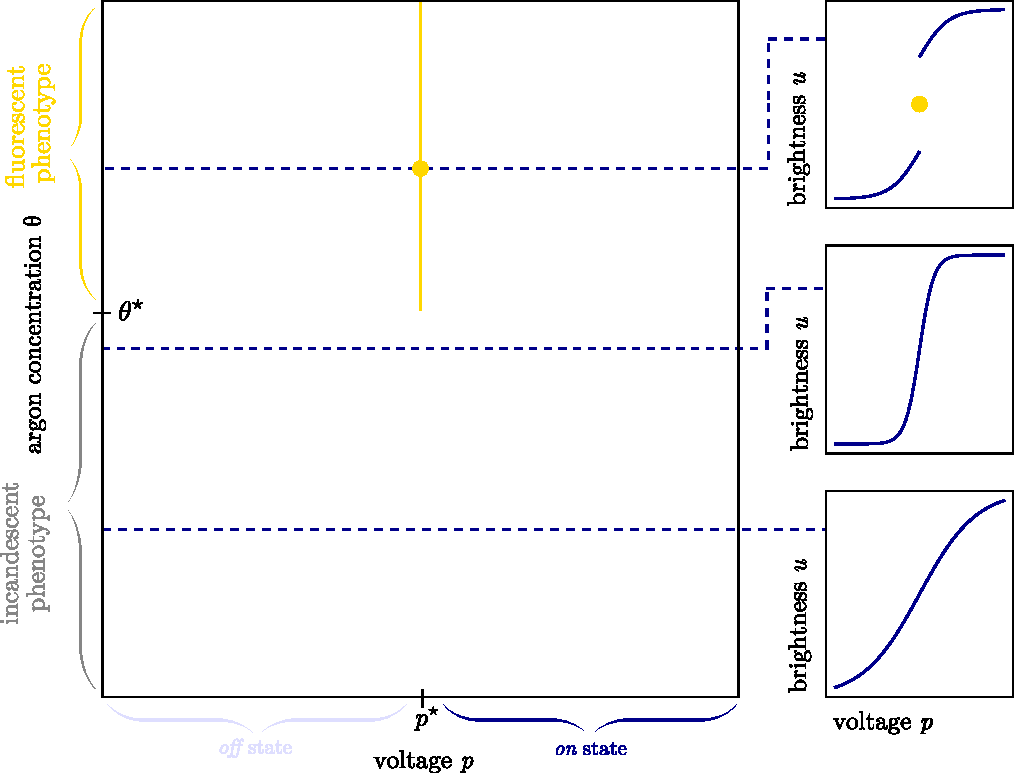
\includegraphics[scale=0.7]{bulb}
\caption{a) The bifurcations (shown in gold) at critical voltage $p^\star$ above argon concentration $\theta^\star$ give rise to sudden jumps in brightness (right-hand panels). $\theta^\star$ separates two bulb phenotypes and $p^\star$ separates the \emph{on} and \emph{off} states.}
\label{fig:bulb}
\end{Figure}

The fluorescent and incandescent bulbs can be considered as two different phenotypes distinguished by the quality of their response to voltage changes. Different colour bulbs can also be considered phenotypes, distinguished by the quality of their \emph{on} state, rather than their response to voltage. Bifurcation theory allows us to describe the transitions between qualitative states and can be leveraged to distinguish and organise phenotypes. In this context a bifurcation becomes a punctuation that either \emph{distinguishes between phenotypes} or \emph{distinguishes between qualitative behaviours within a phenotype}.

Suppose we inserted a component into our light bulb that changed parameter $\theta$ in such a way so that we can change between the discrete response of the fluorescent bulb and the continuous response of the incandescent bulb. Perhaps $\theta$ could be the concentration of argon gas; the bulb would have to be wired to behave like an incandescent bulb at low concentrations. We could collect brightness $u$ as a function of voltage $p$ and gas concentration $\theta$ produce something similar to that shown in Figure \ref{fig:bulb}. The bifurcations at critical voltage $p^\star$ above argon concentration $\theta^\star$ give rise to sudden jumps in brightness. The bifurcations separate the \emph{on} and \emph{off} states of the bulb and are only present in the fluorescent phenotype. The two phenotypes lie either side of  the onset of bifurcations at concentration $\theta^\star$. We can see from Figure \ref{fig:bulb} how knowing the locations of bifurcations allows us to organise qualitative behaviours and hence phenotypes of the bulb.

In the biological context, we can consider changes in $\theta$ as changes in the organism genotype that may or may not lead to a new phenotype. The idea of describing phenotypes in this way has been done before by Waddington \cite{Wang2011QuantifyingDifferentiation,Ferrell2012BistabilityLandscape,Sanchez-Romero2021WaddingtonsWorld}. His epigenetic landscape is a metaphor for how changes gene regulation, in our case represented by changes in $\theta$, determines the fate of cells. He imagines the cell as a marble, rolling down a series of forking valleys representing a differentiation cascade, eventually settling in its final phenotype. Let us adopt this metaphor for organism behaviours in response to a controlled condition (Figure \ref{fig:waddington}). Changing the control condition places the marble at different points in the valley and each fork in the valley corresponds to different available behaviours to the organism. Changing the parameters $\theta$ changes the topology of the valleys potentially giving rise to new behaviours and therefore new phenotypes. We expect that most changes in $\theta$ to either result in very little change in the organism or do nothing at all \cite{Orr2005TheHistory,Khammash2016AnRobustness}. Furthermore most non-neutral mutations are expected to be deleterious \cite{Haag-Liautard2007DirectDrosophila,Eyre-Walker2007TheMutations}. The emerging picture suggests that the route between phenotypes is a carefully created sequence of changes in $\theta$.

\begin{Figure}
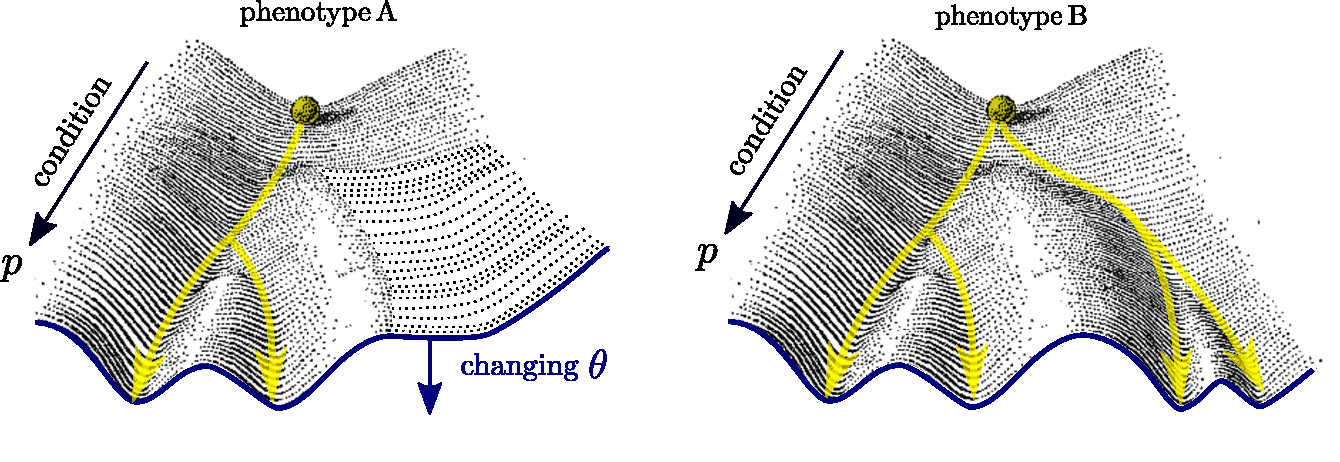
\includegraphics[scale=0.6]{waddington}
\caption{Waddington landscapes representing the set of available behaviours for two phenotypes in response to a controlled condition $p$. Phenotypes are related by changes in landscape topology via changes in $\theta$}
\label{fig:waddington}
\end{Figure}

In order to enumerate the phenotype distribution in the the high-dimensional parameter space $\theta$ for a given organism we can construct a model. By parametrising such a model $\rates(u,p)$ by $\theta$, we can relate the states of the organism $u$ to experimentally controlled conditions $p$. Ideally a subset of $u$ can be observed experimentally so that we may observe bifurcations in the data, as demonstrated in the right-hand panel of Figure \ref{fig:bulb}. In the following section we shall go through a class of models that can leverage bifurcation theory.  

\clearpage
\subsection{Differential Equation Models}

For the purposes of this thesis we will assume that the behaviour of the organism under study can be cast in terms of differential equations in a $N$ states $u$, $M$ parameters $\theta$ and $P$ control conditions $p$. For now we shall state the general class of models and follow up with concrete biological examples as we explore different types of bifurcations. Throughout the thesis we will consider models of the form

\begin{equation}
	\frac{du}{dt} = \rates(u,p)
	\where
	\begin{cases}
		\quad F: \Reals^{N+P}\rightarrow\Reals^N \\
		\quad \theta\in\Reals^M, u\in\Reals^N, p\in\Reals^P
	\end{cases}
	\label{eq:differential-equations}
\end{equation}

\noindent The total derivative $\frac{du}{dt}$ gives us the rate of change of the states with respect to time $t$ and all variables have been vectorised with the appropriate dimension. In principle the right-hand-side $\rates$ can be arbitrarily complicated, containing spatial derivatives or even machine learning models such as neural networks. We shall see later when such models become relevant in biomedical modelling.

\subsubsection{Trajectories \& Field Geometry}

In principle once equations \eqref{eq:differential-equations} have been written down they can be integrated to obtain trajectories $u(t)$ for various initial conditions $u(t')$. We can write the solution down formally as
\begin{equation}
	u(t) = u(t') + \int_{t'}^{t} \rates(u(s),p)\,\mathrm{d}s
	\label{eq:trajectory}
\end{equation}
Here the integral reveals that in order to determine where the state is at time $t$ we need to sum all the contributions of the function $\rates$ from the initial time $t'$ all the way up to final time $t$. The function $\rates$ depends on the state $u$ and must be updated with the integration variable $s$. This calculation can be interpreted, as shown in Figure \ref{fig:fields}, as choosing an initial point $u'=u(t')$ in a vector field $\rates$ and following the field lines until time $t$ at which the final point $u=u(t)$ has been reached.

\begin{Figure}
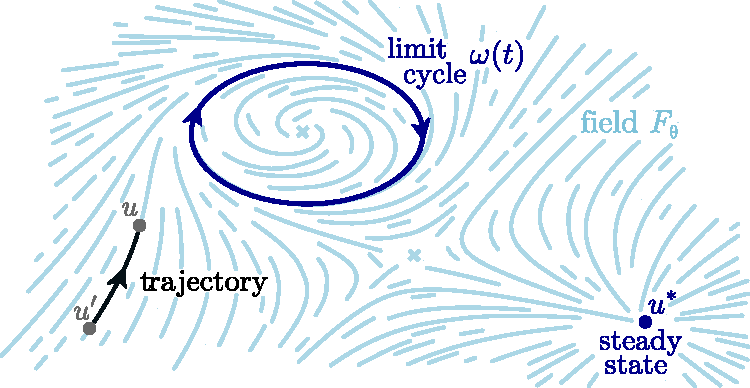
\includegraphics[scale=0.9]{fields}
\caption{Illustration of a trajectory between $u=u(t)$ and $u'=u(t')$ over finite time $t-t'$ following the field lines of $\rates$. In this example field lines either point towards steady state $\steady$ or a limit cycle $\cycle(t)$. There are two unstable fixed points marked by crosses: a saddle point separating the basins of attraction and an unstable focus enclosed by the limit cycle.}
\label{fig:fields}
\end{Figure}

By considering the geometry of the field $\rates$ in state space we can determine the fate of sets of trajectories, which are ultimately pulled towards \emph{dynamical attractors}. Such attractors can be static steady states $\steady$ or dynamic like the limit cycle $\cycle(t)$ illustrated in Figure \ref{fig:fields}. \emph{Dynamical attractors} create basins of attraction defined as regions of state space in which trajectories are pulled towards the same stable structure. These basins must be separated by unstable structures, such as the saddle point marked by a cross in Figure \ref{fig:fields}, which define a boundary between the basins called the separatrix. Note that the direction of the field $\rates$ and not its magnitude $|\rates|$ determines the fate of a trajectories.

When equations \eqref{eq:differential-equations} describe the behaviours of an organism, the attractors determine the set of qualitative behaviours available to the organism of genotype $\theta$, whilst experiencing experimental conditions $p$. If changes to the genotype $\theta$ change the number, type or stability of the attractors then we will observe new qualitative behaviours and hence a new phenotype. If changes to conditions $p$ lead to changes in the state space geometry, this is interpreted as a different behavioural state available to the same phenotype. We can see therefore how casting a biomedical problem into the language of differential equations, allows us to characterise phenotypic traits with the geometry of attractors in state space. 

\subsubsection{The Jacobian Matrix}

In order to quantify the geometry of a local patch of state space $u$ we can imagine $\rates$ as a velocity field of water and place a tiny blob of ink surrounding the location $u$. The so called Jacobian matrix $\jacobian$ of partial derivatives at the location $u$ transforms the basis vectors $\hat u(t)$ defining the blob over a short period of time $\Delta t$ as depicted in Figure \ref{fig:jacobian}. The transformation is
\begin{equation}
	\hat{u}(t+\Delta t)=\left (\mathbb{1}+\jacobian\Delta t \right)\hat{u}(t)
	\where
	\hat{u}\in\Reals^N\quad
	\jacobian\in\Reals^{N\times N}
	\label{eq:jacobian-transformation}
\end{equation}

\begin{Figure}
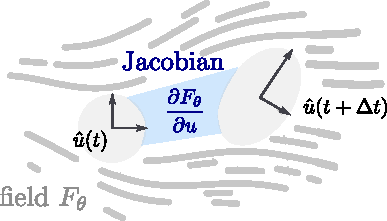
\includegraphics[scale=1.2]{jacobian}
\caption{Illustration how the Jacobian matrix $\jacobian$ transforms the basis vectors $\hat u(t)$ defining a small patch of initial conditions for a short period of time $\Delta t$. The eigenvalues $\lambda$ and eigenvectors $\eigenvector$ define the deformation of the patch}
\label{fig:jacobian}
\end{Figure}
\noindent where $\mathbb{1}$ is the identity matrix. The eigenvalues $\lambda$ and eigenvectors $\eigenvector$ of the Jacobian reveal to us the magnitudes and directions of the stretching or squeezing of the blob. We can diagonalise the Jacobian to obtain the eigenvalues and eigenvectors at any state space location $u$ to quantify the local geometry of the field. The eigenvalue equation is written as

\begin{equation}
	\lambda \eigenvector = \jacobian\eigenvector
	\where
	\eigenvector\in\Reals^N : |\eigenvector|=1
	\label{eq:jacobian-eigenproblem}
\end{equation}
where the eigenvectors are normalised to have unit magnitude. We can take the limit $\Delta t\rightarrow 0$ of equation \eqref{eq:jacobian-transformation} to obtain a first order matrix differential equation for the evolution of basis vectors $\hat u(t)$ in any patch $u$
\begin{equation}
	\frac{d\hat{u}}{dt}=\jacobian\hat{u}
	\label{eq:jacobian-odes}
\end{equation}
The coefficients given by the Jacobian matrix are time-independent and therefore the general solution can be written as a matrix exponential
\begin{equation}
	\hat{u}(t)=\e^{\jacobian(t-t')}\hat{u}(t')
	\label{eq:basis-vector-evolution}
\end{equation}
where $\hat{u}(t')$ are the basis vectors that define the initial shape of the blob centred on location $u$. If we let the basis for the initial blob be parallel to the eigenvectors $\eigenvector$ of the Jacobian, then the evolution any vector $\sigma(t)$ within the blob expressed in its basis becomes the linear superposition
\begin{equation}
	\sigma(t)= \sum_{\lambda}\eigenvector
	\sigma_{\lambda}(t') \e^{\lambda(t-t')}
	\label{eq:eigenbasis-vector-evolution}
\end{equation}
where $\sigma_{\lambda}(t')$ are the initial components of the vector in the basis of the blob. This equation reveals explicitly how the sign of real parts to eigenvalues $\Real\lambda$ determine the exponential growth or shrinkage of the blob in the direction $\eigenvector$. The imaginary parts $\Imag\lambda$ determine the magnitude of rotations of the blob. Note that since the Jacobian matrix is real and eigenvalues and eigenvectors appear in conjugate pairs and therefore the overall evolution \eqref{eq:eigenbasis-vector-evolution} yields real transformations of blob vectors $\sigma(t)$. The transformation \eqref{eq:jacobian-transformation} an approximation of the time-ordered exponential transformation \cite{Bauer2012Time-OrderingExpansion} and we should note that the results stated here are valid for small blobs $|\sigma(t)|\ll 1$ over short timescales $|t-t'|\ll1$.

\subsubsection{Time Ordered Exponetials}

In this section we go a bit deeper into the origin of transformation \eqref{eq:jacobian-transformation} for those who are interested the evolution of state space blobs over arbitrary time intervals. We begin by considering the evolution of the separation between a trajectory $u(t)$ and its perturbation $u(t)+\delta u(t)$
\begin{equation}
	\frac{d}{dt}(u+\delta u) = \rates(u+\delta u,p)
\end{equation}
After Taylor expanding the field $\rates$ and recognising that equations \eqref{eq:differential-equations} lead to a cancellation in the terms involving the unperturbed trajectory $u$ we arrive at
\begin{equation}
	\frac{d}{dt}(\delta u) =
	\left.\jacobian\right|_{u=u(t)}\!\!\delta u + \mathcal{O}(\delta u^2)
	\label{eq:linearised-differential-equations}
\end{equation}
where $\jacobian$ is the Jacobian of the field and additional terms $\mathcal{O}(\delta u^2)$ involve taking higher order derivatives of the field $\rates$. Choosing a perturbation sufficiently small such that we can ignore higher order terms yields a first order homogenous ordinary matrix differential equation of the form $\dot{\delta u}(t)\approx J(t)\delta u(t)$ where $J(t)$ is a time-varying Jacobian. These equations can be solved formally with time-ordered matrix exponentiation \cite{Bauer2012Time-OrderingExpansion} 

\begin{Figure}
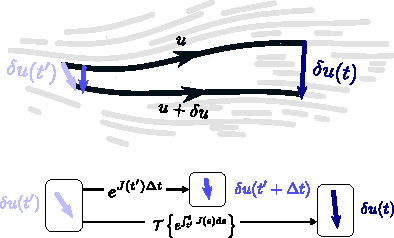
\includegraphics[scale=1.5]{lyapunov}
\caption{Illustration how the time ordering operator $\mathcal{T}\left\{\e^{\int_{t'}^t J(s) \mathrm{d}s}\right\}$ propagates the separation $\delta u(t)$ between adjacent trajectories $u$ and $u+\delta u$ by repeated application of the exponentiated Jacobian $\e^{J(t)\Delta t}$ evaluated along trajectory $u(t)$}
\label{fig:lyapunov}
\end{Figure}
\begin{equation}
	\delta u(t) \approx
	\mathcal{T}\left\{\e^{\int_{t'}^t J(s) \mathrm{d}s}\right\}\delta u(t')
	\where
	J(t) := \left.\jacobian\right|_{u=u(t)}
	\label{eq:matrix-exponential}
\end{equation}
The time-ordering defines an ordered product of matrix exponentials
\begin{equation}
	\mathcal{T}\left\{ \e^{\int_{t'}^t J(s) \mathrm{d}s} \right \}:=
	\lim_{\Delta t\rightarrow 0}\left(
		\e^{J(t)\Delta t}\e^{J(t-\Delta t)\Delta t}\,\dots\,
		\e^{J(t'+\Delta t)\Delta t}\e^{J(t')\Delta t}
	\right)
	\label{eq:time-ordering-operator}
\end{equation}
which can be calculated by repeated exponentiation of the Jacobian $\e^{J(t)\Delta t}$ evaluated at different times along the unperturbed trajectory $u(t)$. Although this expression may look complicated it is just another matrix whose eigenvalues reveal whether the trajectories diverge $|\delta u(t\rightarrow\infty)|\rightarrow\infty$ or converge $|\delta u(t\rightarrow\infty)|\rightarrow0$.

In situations where we want to investigate field flow over longer time intervals or where there is an explicit time dependence in the field $\rates(u,p,t)$ we must use the time-ordered exponential \eqref{eq:time-ordering-operator} in place of the exponentiated Jacobian.

\subsubsection{Lyapunov Exponents}
Sometimes we are only interested in the rate of change of the magnitude of deformations $|\sigma(t)|$ which can quantified by the \emph{finite time lyapunov exponent}
\begin{equation}
	\Lambda(u,\Delta t):=\frac{1}{\Delta t}\log\frac{|\sigma(t+\Delta t)|}{|\sigma(t)|}
\end{equation}
We remind ourselves that the blob $\sigma(t)$ is centred around state space point $u$, then evolved for a time $\Delta t$ and therefore the exponent is a function of $\Delta t$ and $u$. Substituting equation \eqref{eq:eigenbasis-vector-evolution} we arrive at
\begin{equation}
	\Lambda(u,\Delta t) = \frac{1}{2\Delta t}\log
	\left\langle
		\e^{2\Real[\lambda]\Delta t}
	\right\rangle_{\sigma(t)}
	\ge 
	\left\langle
		\Real[\lambda]
	\right\rangle_{\sigma(t)}
	\label{eq:finite-time-lyapunov}
\end{equation}
where $\left\langle\cdots\right\rangle_{\sigma(t)}$ is a shorthand for a weighted arithmetic average over the components of the initial blob $\sigma(t)$. We have used Jensen's Inequality \cite{ValeursMoyennes1906SurMoyennes} to show that the rate of distortions is bounded by the average of real parts of eigenvalues. This bound becomes an equality for eigenvalue $\lambda$ when the blob $\sigma(t)$ is initialised along only its eigenvector $\eigenvector$. We will see later how the \emph{Lyapunov exponents} are useful for extracting timescales around interesting structures in state space such as \emph{fixed points} and \emph{degeneracies}. 

\subsubsection{Fixed Points}

Thus far we explored the field geometry in arbitrary patches of state space $u$ and asked questions about local flows. It is usually not possible to set up experimental conditions to get an organism to trace out all of its available states without killing it or distorting the mechanism under study. An organisms prefers to operate within a finite set of states and would want to return to them when perturbed. In biology this is known as \emph{homeostasis} and in the context of dynamical systems this is a stable steady state $\steady$ which belongs to a wider class of points called \emph{fixed points}. In the context of differential equation models, a \emph{fixed point} is the solution of
\begin{equation}
	\left.\frac{du}{dt}\right|_{u=\steady}=\rates(\steady,p) = 0
	\label{eq:fixed-point-equation}
\end{equation}

\begin{Figure}
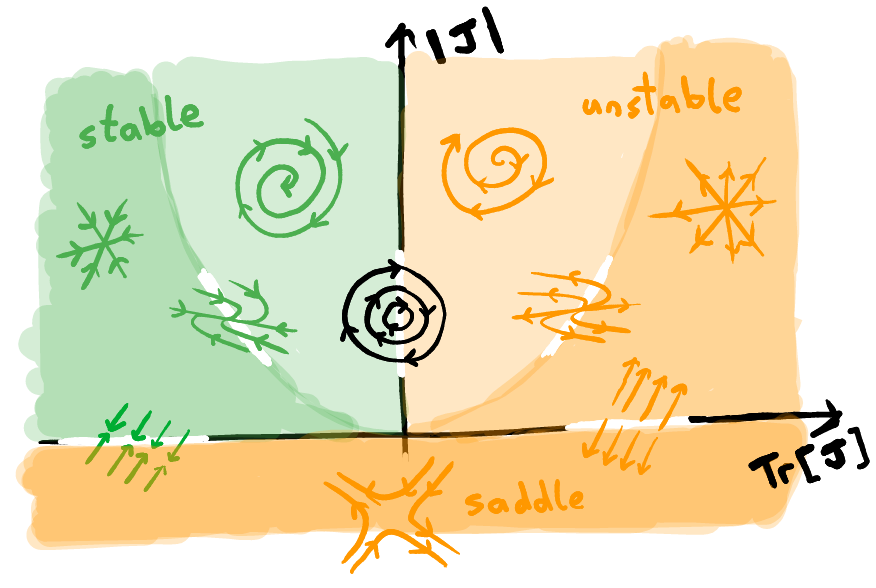
\includegraphics[scale=0.35]{stability}
\caption{Classification of stable and unstable fixed points for a general two dimensional systems in terms of trace $\mathrm{Tr}[\jacobian]$ and determinant $|\jacobian|$ of its Jacobian}
\label{fig:stability}
\end{Figure}

By looking at the eigenvalues of the Jacobian, which determine local flows according to equations \eqref{eq:eigenbasis-vector-evolution}, we can classify the fixed point $\steady$. The sign of real parts $\Real\lambda$ determine whether small perturbations away from the fixed point will diverge. This defines whether the point is \emph{stable}, \emph{unstable} or a \emph{saddle}. Non-zero imaginary parts $\Imag\lambda \ne 0$ give rise to damped oscillation around the point; these points are called \emph{foci}. Without real parts the flow becomes purely rotational and give rise to \emph{cycles}.

For a two dimensional system we can express the two eigenvalues of the $2\times 2$ Jacobian in terms of its trace $\mathrm{Tr}[\jacobian]$ and determinant $|\jacobian|$ which allows us to conveniently reveal all the possible fixed points types, as in Figure \ref{fig:stability}. If at least one the eigenvalues vanishes the fixed point becomes \emph{degenerate}. We shall see that \emph{degenerate} field flows lead to critical slowing down in dynamics, reveal bifurcations and are useful for constructing tangent fields to implicitly defined surfaces.

\subsubsection{Field Degeneracy}
\label{section:field-degeneracy}
A field $\rates$ can be called \emph{degenerate} where it is locally constant and hence does not cause shape changes to a blob of initial conditions in one or more directions. This means that one or more of the eigenvalues of the Jacobian vanish $\lambda = 0$ and have associated eigenvectors $\hat T_\lambda$ tangent to the direction where the field is locally constant. Suppose the field is \emph{degenerate} at point $\degenerate$, then the vanishing eigenvalues lead to a zero determinant $\left|\jacobian\right|=0$ and the eigenvectors must be orthogonal to all the gradients
\begin{equation}
	\left|\jacobian\right|_{u=\degenerate} \!\!\! = 0
	\qquad\left.\jacobian\right|_{u=\degenerate}\!\!\!\hat T_\lambda = 0
	\where
	\hat T_\lambda\in\Reals^N : |\hat T_\lambda|=1
	\label{eq:degeneracy-conditions}
\end{equation}
The eigenvector equation yields $\hat T_\lambda$ that span the degenerate subspace at field location $\degenerate$. The number of vectors and hence the size of the subspace is given to us by the number of vanishing eigenvalues $\lambda=0$. In linear algebra this would be referred to as the \emph{nullspace} or \emph{kernel} of the Jacobian matrix. A vanishing determinant means that the Jacobian is not invertible.

\subsubsection{Critical Slowing Down}
% A fixed point $\steady$ that is also degenerate $\degenerate$ is called a critical point $\critical$. This is a location in the state space that satisfies equations \eqref{eq:fixed-point-equation} and \eqref{eq:degeneracy-conditions}. This means that the field $\rates$ is not only zero, but also locally zero along at least one direction. In this case the whole degenerate subspace takes on the character of the fixed point and gives rise to power law timescales that are characterised using \emph{critical exponents}.

% \emph{Critical exponents} are not the same as \emph{Lyapunov exponents} although we will see that they are related. These exponents are important because the power laws can be detected in trajectory data and can be used to classify bifurcations.

Lets us consider the magnitude of deformations along the degenerate direction $T_\lambda(t)$ in the vicinity of the the region $u\approx\degenerate$ that is driven by the scalar sub-field $F_\lambda$. We expect the first-order derivatives to vanish $\left.\frac{dF_\lambda}{dT_{\lambda}}\right|_{u=\degenerate}\!\!\!\!\!\!\!\!\!\!\!\!\!\!\!=0$ and therefore have to expand the field $F_\lambda$ to an order $n$ that will yield the first non-zero derivative. The equations expanded for $u\approx\degenerate$ are
\begin{align}
	\frac{d T_\lambda}{dt} &= \left.\frac{dF_\lambda}{dT_{\lambda}}\right|_{u\approx\degenerate}
	\!\!\!\!\!\!\!\!\!\!\!\!T_\lambda(t) +
	\frac{1}{n!}
	\left.\frac{d^n F_\lambda}{dT_{\lambda}^n}\right|_{u\approx\degenerate}
	\!\!\!\!\!\!\!\!\!\!\!\!T_{\lambda}(t)^n +\mathcal{O}(T^{n+1})
	\where n \ge 2
	\label{eq:bernoulli-differential-equation}
\end{align}
Here we kept the first-order derivative because we would still like to see how the dynamics scales with time as we approach to degeneracy. This is a Bernoulli differential equation \cite{1993SolvingI} with constant coefficients and has a general solution
\begin{align}\!\!\!\!\!
	T_{\lambda}(t) = \left(
	\left(T_{\lambda}(t')\e^{(t-t')
	\left.\frac{dF_\lambda}{dT_{\lambda}}\right|_{u\approx\degenerate}
	}\right)^{1-n}
	-(t-t')\frac{n-1}{n!}\left.\frac{d^n F_\lambda}{dT_{\lambda}^n}\right|_{u\approx\degenerate}
	\right)^{\frac{1}{1-n}}
	\label{eq:critical-slowing}
\end{align}

This equation reveals two timescales for blob deformations in the vicinity of a field degeneracy: the familiar exponential timescale $\e^{t-t'}$ and a new polynomial timescale $(t-t')^{\frac{1}{1-n}}$. The emergence of a polynomial timescale that dominates over the exponential is called \emph{critical slowing down} and is a marker of degeneracy. We can see once the dynamics is confined to the degenerate subspace the eigenvalues of the Jacobian are insufficient for determining the timescales. The curvature of the field around the degenerate subspace drives the polynomial dynamics, and therefore higher-order derivatives are needed to reveal this.

This critical slowing can be observed in data when \emph{fixed points} become \emph{degenerate}. Degenerate fixed points are also called \emph{critical points}. The transition between these two timescales in data is a signal that a \emph{critical point} is nearby. We will see that \emph{critical points} may lead to bifurcations and are accompanied by degeneracies in the field known as centre manifolds \cite{Carr1981ApplicationsTheory}.

\subsubsection{Fluctuations}
\label{section:fluctuations}

Biological processes can be intrinsically noisy and the measurement apparatus can also introduce errors. Fortunately we can model such non-deterministic aspects by extending equations \eqref{eq:differential-equations} to a Langevin equation
\begin{align}
	\frac{du}{dt} = \rates(u,p) + \eta(t)
	\where \eta(t) \sim \mathcal{N}(\mu=0,\mathbf{\Sigma}=\mathbb{1}D)
	\label{eq:langevin}
\end{align}
The stochastic process $\eta(t)$ is a zero-mean white noise with equal variance $D$ along all $N$ dimensions resultant from a large number of independent processes such as Brownian motion and Poisson shot noise. We can apply the Kramers-Moyal expansion \cite{Kramers1940BrownianReactions} to transform this equation into an equivalent Fokker-Planck equation for the probability distribution $P_{\theta}$
\begin{align}
	\frac{dP_{\theta}}{dt} + \frac{\partial}{\partial u}\cdot J_\theta = 0
	\where J_\theta := \left(\rates(u,p)-\frac{D}{2}
	 \frac{\partial}{\partial u} \right)P_{\theta}
	\label{eq:fokker-planck}
\end{align}
Here we cast the Fokker-Planck equation as a continuity equation with the divergence of probability current $J_\theta$ balancing the total change in probability $\frac{dP_{\theta}}{dt}$. In the scenario where at steady state $\frac{dP_{\theta}}{dt}=0$ there are also no circulating probability currents $J_\theta=0$ then we can solve for the distribution
\begin{align}
	P_{\theta}(u,p) = \frac{1}{Z} \mathbb{e}\,^{\frac{2}{D}\int^{u}\!\!\!\rates(u',p)\cdot\mathrm{d}u'}
	\where Z:= \int_{\Reals^N} \mathbb{e}\,^{\frac{2}{D}\int^{u}\!\!\!\rates(u',p)\cdot\mathrm{d}u'} \mathrm{d}u
	\label{eq:steady-state-distribution}
\end{align}
Expanding the distribution in the vicinity of a stable fixed point gives rise to a multivariate Gaussian distribution whose covariance matrix $\mathbf{\Sigma}$ is the inverse of the Jacobian evaluated at the fixed point
\begin{align}
	P_{\theta}(u,p) \sim \mathbb{e}\,^{-\frac{1}{2}
	(u-\steady)^\top\mathbf{\Sigma}^{-1}(u-\steady)
	}\where \mathbf{\Sigma}^{-1}=-\frac{2}{D}\left.\jacobian\right|_{\steady}
	\label{eq:steady-state-distribution-near-fixed-point}
\end{align}
We learn that accompanying the \emph{critical slowing down} \eqref{eq:critical-slowing} we also have the divergence of variance along the degenerate direction. These are the two main observations that accompany bifurcations and have a deep relationship to the theory of phase transitions \cite{Bose2019BifurcationCriticality}.

\subsubsection{Limit Cycle Analysis}
Thus far we dealt with static state space structures like \emph{fixed points}. We found that the eigenvalues of the Jacobian are sufficient for their characterisation, unless the field is  \emph{degenerate}, in which case higher order derivatives of the field must be investigated.

If fields lines point towards a region of state space but the region \emph{does not} contain any fixed points, then the only other option is for the field lines to converge onto a \emph{limit cycle}. This is actually a rough statement of the Poincar\'e-Bendixson theorem \cite{Ciesielski2012TheCentury}  which allows us to define trapping regions where trajectories do not escape from and make statements about the existence or non-existence of limit cycles. Limit cycles also enclose a finite number of \emph{unstable foci} that push trajectories away from their centers.
\begin{Figure}
	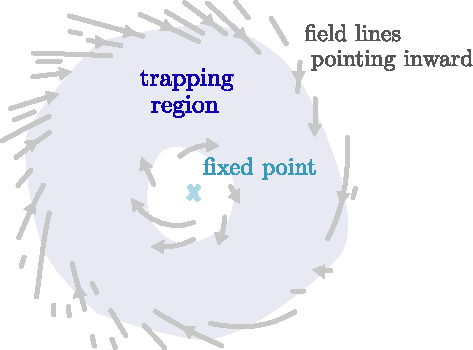
\includegraphics[scale=0.9]{limit-cycle}
	\caption{Conditions of a limit cycle as determined by the Poincar\'e-Bendixson theorem. A region with no fixed points and all fields lines pointing inward/outward must contain a stable/unstable limit cycle.}
	\label{fig:limit-cycle}
\end{Figure}
Newton-type methods can easily be applied to find \emph{fixed points} because they are local structures in fields. Limit cycles are much more tricky because it is not possible to know whether a local state part of a limit cycle or not before we have seen a trajectory visit that state twice: once at $u(t)$ and then again $u(t+T)$ after some time $T$. Limit cycles are inherently global structures in state space. Limit cycles can be computed by some form of discretisation or meshing of the recurrence condition, with methods such as trapezoid \cite{Lust2000ComputationSystems,Uecker2018HopfApplications}, collocation \cite{Kuznetsov2004NumericalBifurcations} and shooting \cite{Lust2000ComputationSystems}.

\clearpage
\subsection{Bifurcation Analysis}
\label{section:bifurcation-analysis}
We have surveyed sufficiently many state space structures, the geometry of which determine the qualitative behaviour of the organism we are describing. An organism has many qualitative behaviours in response to conditions $p$ and many phenotypes emerging from changes in $\theta$.

Bifurcations are defined as qualitative changes to system behaviour in response to smooth changes to some conditions. This means that as conditions change, state space structure will merge, split and change geometry. In our setting these conditions could be either $\theta$ or $p$, but we will focus on changes with respect to $p$ with the understanding that the analysis is equally valid for $\theta$. Changes to state space structures, and hence bifurcations can be \emph{local} or \emph{global}.

\begin{Figure}
	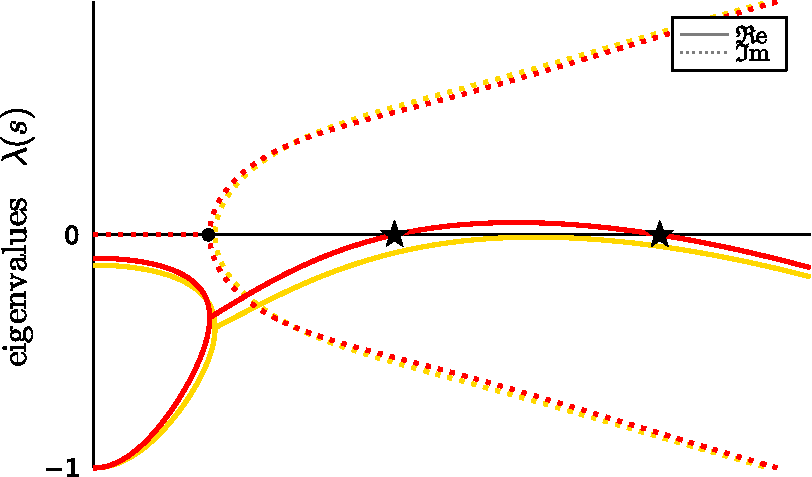
\includegraphics[scale=0.6]{local-bifurcations} 
	\caption{A \emph{local} bifurcation at $(u^\star,p^\star)$ can be detected by tracking the sign of the real parts $\Real[\lambda]$ of Jacobian eigenvalues as a function of control condition $p$}
	\label{fig:local-bifurcations}
\end{Figure}

We shall first focus on \emph{local} bifurcations that can be analysed by investigating the eigenvalues of the Jacobian at a specific point $(u^\star,p^\star)$. A \emph{local} bifurcation point $(u^\star,p^\star)$ is in fact a \emph{critical point} in the field $\rates$: a fixed point $\rates(u^\star,p^\star)=0$ where at least one Jacobian eigenvalue crosses the imaginary axis $\Real[\lambda]=0$ with a finite slope. The number of eigenvalues that cross the imaginary axis defines the dimensionality of the centre manifold along which the bifurcation occurs \cite{Carr1981ApplicationsTheory}. Furthermore, it is the eigenvalue with largest real part that determines the stability of a fixed point and thus it is sufficient to consider the behaviour a single eigenvalue. The number of parameters $p$ that need to be varied defines the \emph{co-dimension} of the bifurcation. Sometimes a bifurcation also \emph{degenerate} in which case eigenvalues cross the imaginary axis with vanishing slope. In this setting the Jacobian does not reveal enough information about the \emph{critical point} and higher-order derivatives in the field $\rates$ are needed. \emph{Global} bifurcations cannot be determined by local stability analysis at specific points $(u^\star,p^\star)$ alone. We shall see how additional \emph{global} constrains are needed that reveal the formation or changes in limit sets. We present the \emph{supercritical} cases of bifurcations in the following sections, with the understanding that \emph{subcritical} cases can be recovered by reversing the flow in state space.

\subsubsection{Generic Robust Bifurcations}
\label{fig:robust-local-bifurcations}
We are ready to present the two \emph{generic} and \emph{robust} co-dimension one bifurcations: the \emph{saddle-node} (Figure \ref{fig:saddle-node}) and \emph{Hopf} (Figure \ref{fig:hopf}) bifurcation. These bifurcations are generic in the sense that they happen in $N$ dimensional systems, but can be described as happening along one dimension. The bifurcations are \emph{robust} in the sense that small changes to system parameters do not destroy the bifurcation. This is not the case for \emph{pitchfork} and \emph{transcritical} bifurcations. The \emph{pitchfork} (Figure \ref{fig:pitchfork}) and \emph{transcritical} (Figure \ref{fig:transcritical}) bifurcations are co-dimension one examples where small perturbations in condition $p$ split the bifurcations into \emph{saddle-nodes}.
\subsubsection{Global Bifurcations}
\label{section:global-bifurcations}
While \emph{global} bifurcations still happen at a specific condition $p^\star$ there is no single location $u^\star$ at which it happens. Instead we need to track the behaviour of a whole set $\partial\Omega$ in state space. The \emph{cyclic fold} (Figure \ref{fig:cyclic-fold}) and \emph{homoclinic} (Figure \ref{fig:homoclinic}) bifurcations are co-dimension one examples where while the stability of fixed points does not change, a limit set $\partial\Omega$ is created or destroyed. The \emph{infinite period} (Figure \ref{fig:infinite-period}) bifurcation locally appears as a \emph{saddle-node}, but in fact controls the appearance of a limit cycle. The limit cycle becomes evident when trajectories that are pushed away by the saddle point return back to the saddle-point from its stable directions.

\begin{Figure}
	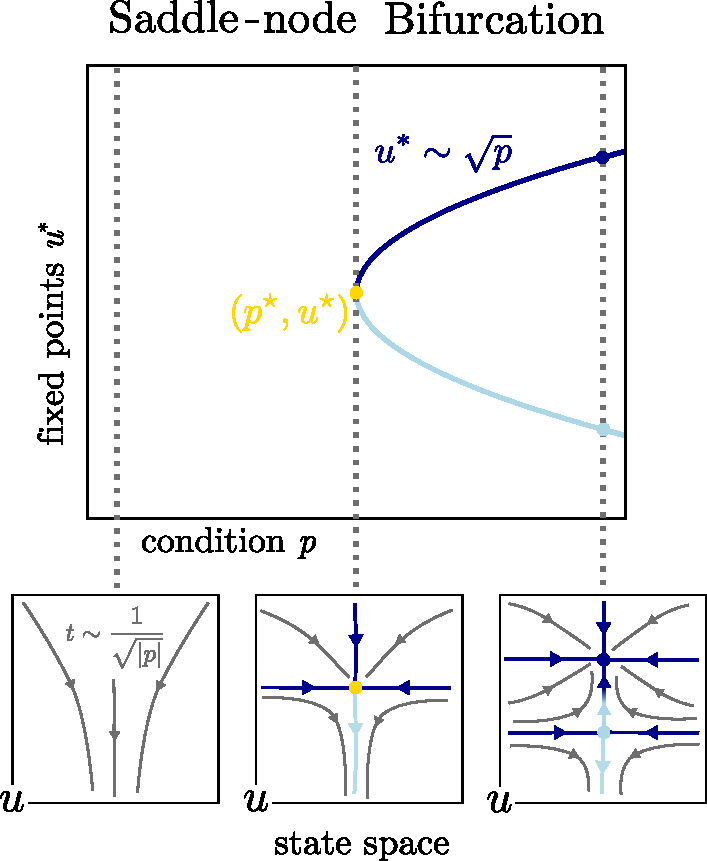
\includegraphics[scale=0.6]{saddle-node} 
	\caption{The \emph{saddle-node} bifurcation creates or annihilates stable and unstable pairs of fixed points. A critical slow-down that scales like $t\sim\frac{1}{\sqrt{|p-p^\star|}}$ can be used to detect its onset.}
	\label{fig:saddle-node}
\end{Figure}

\begin{Figure}
	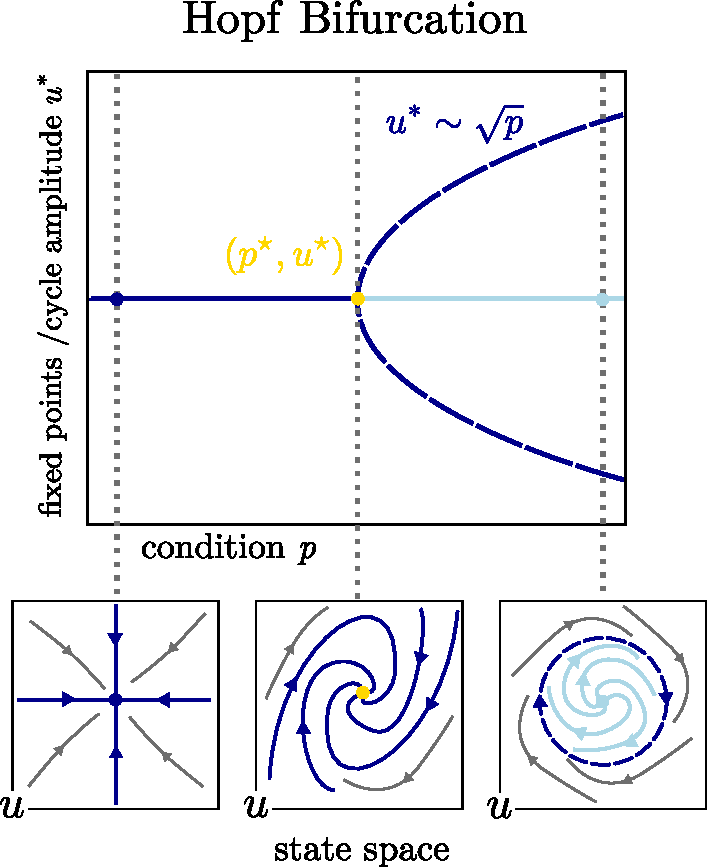
\includegraphics[scale=0.6]{hopf}
	\caption{In a \emph{Hopf} bifurcation a stable fixed point becomes an unstable focus that pushes trajectories towards a limit cycle, subject to conditions of the Poincar\'e-Bendixson theorem. The limit cycle amplitude grows as $\sqrt{p-p^\star}$}
	\label{fig:hopf}
\end{Figure}

\begin{Figure}
	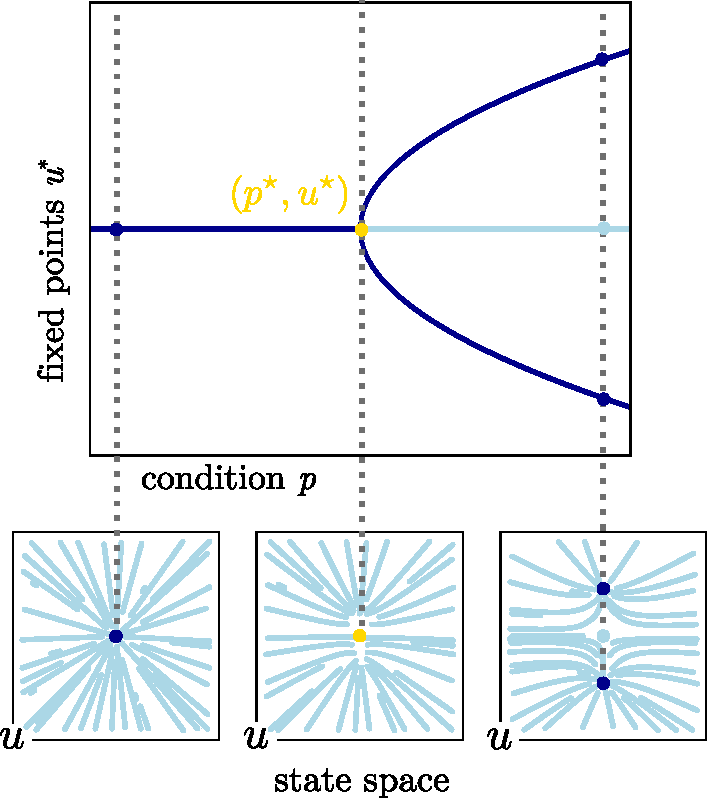
\includegraphics[scale=0.6]{pitchfork}
	\caption{In \emph{Pitchfork} bifurcations a single stable fixed point splits into two stable fixed points separated by a saddle point. The distance between points grows as $\sqrt{p-p^\star}$. Small perturbations in $p$ breaks the pitchfork into a \emph{saddle node} bifurcation and a stable branch of fixed points.}
	\label{fig:pitchfork}
\end{Figure}

\begin{Figure}
	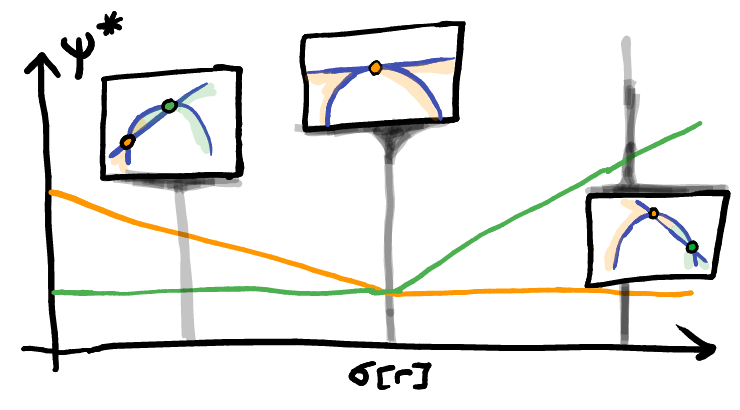
\includegraphics[scale=0.6]{transcritical}
	\caption{In \emph{transcritical} bifurcations a stable and unstable fixed point collide and exchange stability. The distance between points grows as $p-p^\star$. Small perturbations in $p$ breaks the transcritical into two \emph{saddle-node} bifurcations.}
	\label{fig:transcritical}
\end{Figure}

\begin{Figure}
	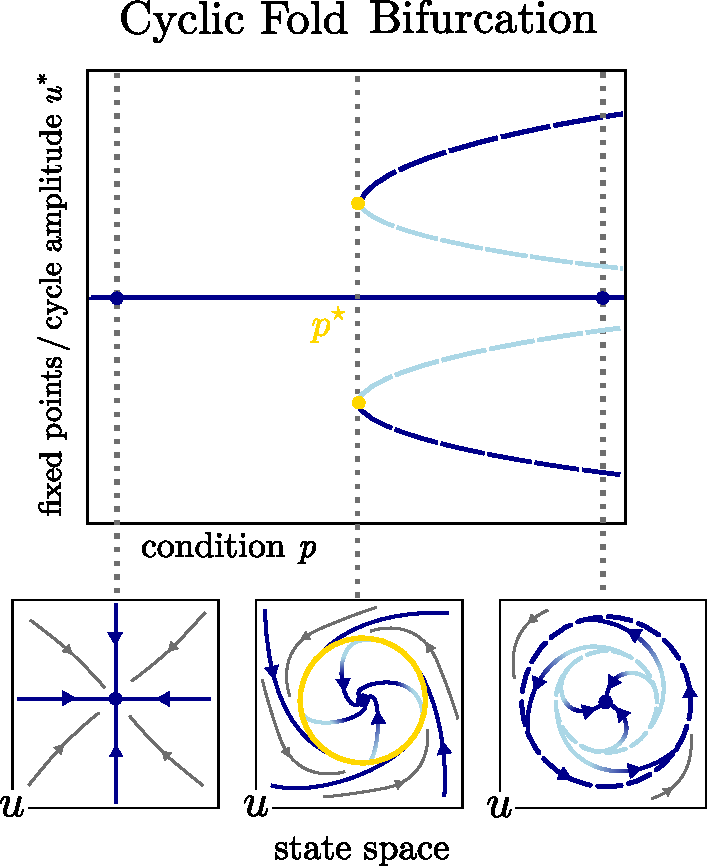
\includegraphics[scale=0.6]{cyclic-fold}
	\caption{The \emph{cyclic fold} bifurcation is a \emph{global} bifurcation that creates or annihilates stable and unstable pairs of limit cycles.}
	\label{fig:cyclic-fold}
\end{Figure}

\begin{Figure}
	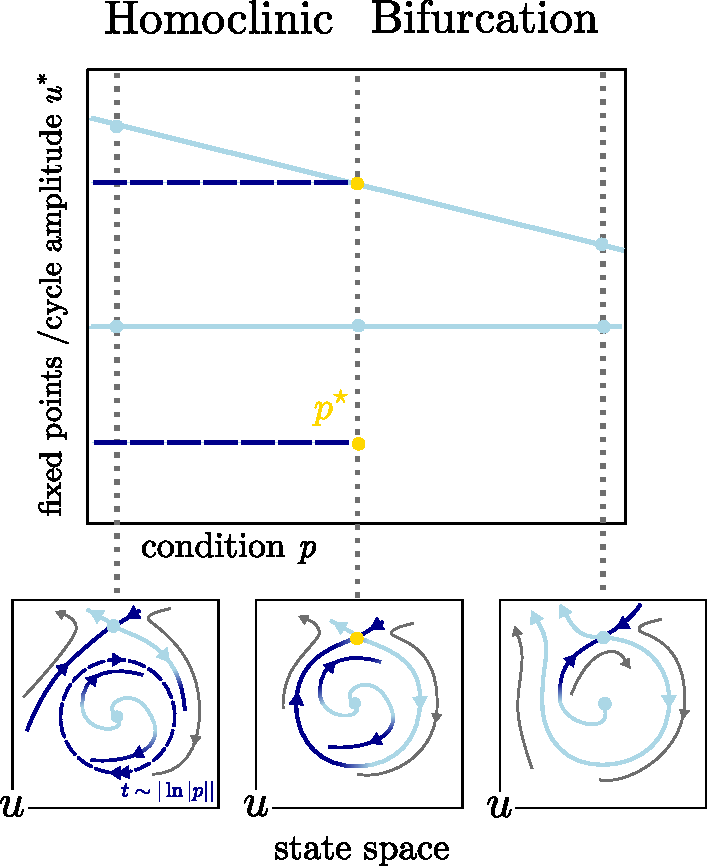
\includegraphics[scale=0.6]{homoclinic}
	\caption{A \emph{homoclinic} bifurcation occurs when a saddle point collides with a limit cycle, forming a \emph{homoclinic} orbit just before breaking the cycle. It is accompanied by a period slow-down that scales like $t\sim|\log|p-p^\star||$}
	\label{fig:homoclinic}
\end{Figure}

\begin{Figure}
	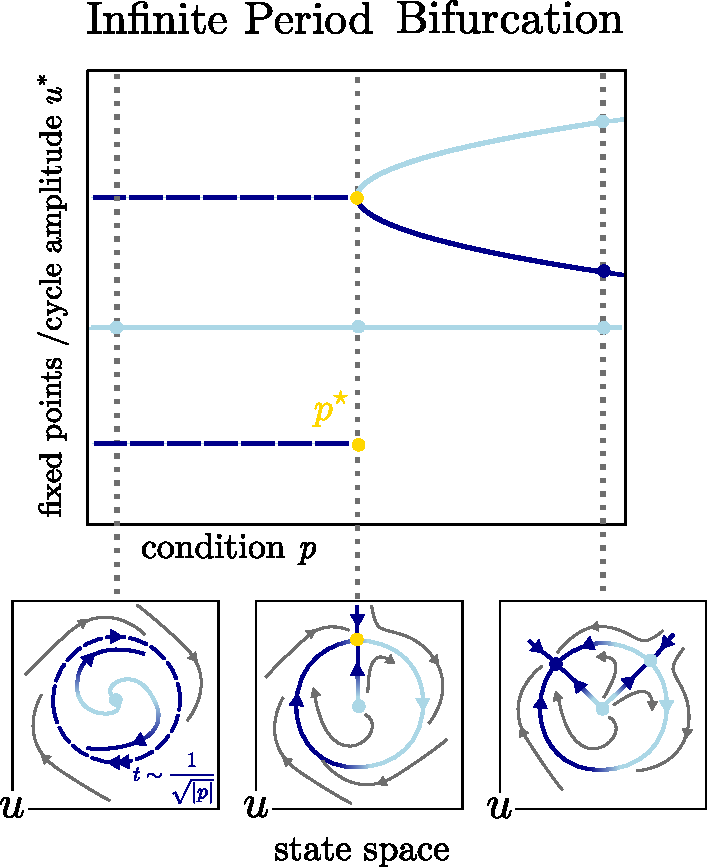
\includegraphics[scale=0.6]{infinite-period}
	\caption{The \emph{infinite period} bifurcation is a \emph{global} bifurcation where a \emph{saddle-node} bifurcation occurs along the limit set, breaking the cycle. It is accompanied by a period slow-down that scales like $t\sim\frac{1}{\sqrt{|p-p^\star|}}$}
	\label{fig:infinite-period}
\end{Figure}

\subsubsection{Normal Forms \& Higher Co-dimension}
In this introduction we provided a geometrical understanding of co-dimension one bifurcations and would like to re-direct the reader the popular book by Steven Strogatz \cite{Strogatz2000} for mathematical details and higher co-dimension bifurcations such as \emph{cusp} and \emph{Bogdanov-Takens}. The normal forms are essentially taylor expansions of the field $\rates$ around \emph{local} bifurcation points.

\subsubsection{Numerical Methods}
In this thesis we extensively use Julia; the library \texttt{DifferentialEquations.jl} \cite{Rackauckas2017Differentialequations.jlJulia} for numerically solving differential equations and \texttt{BifurcationKit.jl} \cite{Veltz2020BifurcationKit.jl} for calculating bifurcation diagrams. \texttt{DifferentialEquations.jl} implements state-of-the-art, well-optimized ordinary and partial differential equation solvers which routinely outperform the "standard" C/Fortran methods and algorithms optimized for high-precision and high-performance computing applications \cite{}. \texttt{BifurcationKit.jl} aims at performing automatic bifurcation analysis of possibly large dimensional equations $\rates(u,p)=0$ where $p\in\Reals$ by taking advantage of iterative methods, sparse formulation and GPU-acceleration. It incorporates continuation algorithms such as pseudo-arclength continuation \cite{} and deflated continuation \cite{}. A Newton-Krylov method \cite{} is used to correct the predictor step and a matrix-free eigensolver \cite{} is used to compute stability and localise bifurcation points. Additionally, periodic orbit computation and continuation using the shooting \cite{}, finite-difference \cite{} and collocation \cite{} methods are implemented. Details of these algorithms can also be found in in the documentation of the above mentioned Julia packages.

\subsection{Spatially Extended Systems}
Suppose we wanted to model the spatial distribution biochemicals across an organism, a population of cells or perhaps even within the cell. Our model $\rates$ would have to contain spatial derivatives and we would supply additional conditions on $u$ with respect to spatial variables $x$ to give a unique solution $u(x,t)$ to the resulting partial differential equation. When studying spatio-temporal dynamics of organisms, a popular choice is to incorporate a diffusive term that models the exchange of matter between spatial locations, giving rise to a \emph{reaction-diffusion} equation
\begin{equation}
	\frac{\partial u}{\partial t} = \rates(u,p) + D\frac{\partial^2 u}{\partial x^2}
	\label{eq:reaction-diffusion}
\end{equation}
where diagonal matrix $D\in\Reals^{N\times N}$ encodes the spatial mobility of each component. Depending on the spatial scale that is being modelled the components of $D$ will take on a different meaning. If we are modelling a population of cells then the components of $D$ quantify which components the cells can exchange between each other. If we are modelling the spatial distributions within a single cell, then $D$ encodes for components that are passively transported between locations. In order to model active transport we would include a first-order spatial derivative term, giving rise to an \emph{advection-reaction-diffusion} equation \cite{}. Although the inclusion of spatial derivatives and boundary conditions may seen quite complicated, we can rest assured that ultimately the discretisation of any partial differential equation will yield a matrix representation of the spatial derivative. Any partial differential equation with $N$ components can be discretized into $K$ spatial grid-points and re-cast as a set of $N\times K$ ordinary differential equation.

\subsubsection{Eigenvalue Distributions of Derivative Operators}
Using the Circular Diagonalization Theorem \cite{} one can derive the eigenvalues $\lambda_k$ of an $K\times K$ matrix which represents the second-order central difference approximation to the second derivative on $K$ sites of a one dimensional ring
\begin{align}
	\frac{\partial^2}{\partial x^2} \rightarrow
	\begin{pmatrix}
	  -2 & 1 &  &  &  & 1 \\
	  1 & -2 & 1 &  &  &  \\
	  & 1 & \ddots & \ddots &  & \\
	  & & \ddots & \ddots & 1 & \\
	  & & & 1 & -2 & 1 \\
	  1 & & & & 1 & -2 \\
	\end{pmatrix}\\
	\begin{matrix}
	  \lambda_k =2\left(\cos\left(\frac{2\pi k}{K}\right)-1\right) \\
	  k\in\{0,1,\cdots,K-1\}
	\end{matrix}
	\qquad
\end{align}
As the number of sites $K\rightarrow\infty$ the argument $k/K\in[0,1]$
and the eigenvalues remain bounded $-4<\lambda_k<0$. By shifting and scaling
the index $k\rightarrow\frac{k-K\pi}{2\pi}$ the eigenvalues are expressed as
a dispersion relation
\begin{align}
  \lambda(k)&=
  -2\left(\cos k+1\right)
  \quad k\in[-\pi,\pi]
\end{align}
The discrete $L$-dimensional laplacian is simply the kronecker sum $\oplus$ of one
dimensional cases and thus its eigenvalues is simply the sum one dimensional dispersions \cite{}
\begin{align}
  \lambda(k)&=
  -2\sum_{i=1}^L\left(\cos k_i+1\right)
  \quad k\in[-\pi,\pi]^L
\end{align}
The probability density $P(\lambda)$ can be expressed as a density integral
over the $L$-dimensional hypercube region $[-\pi,\pi]^L$
\begin{align}
	P(\lambda')&=\frac{1}{Z}\int_{[-\pi,\pi]^L}\!\delta(\lambda'-\lambda(k))\,\mathrm{d}k
\end{align}
We proceed with an element-wise change of variables $u=2\cos k$ and recognise that the integration region is $L$-fold symmetric across each component axis, which allows restriction of the domain of integration to a hyper-octant. In coordinates $u$ the region becomes $[-2,2]^L$
\begin{align*}
  P(\lambda)&=\frac{1}{Z}
  \int_{\Omega'}\!
  \frac{\delta(\Lambda_L+\sum_{u\in\bar{\mathbf{u}}}u)}
  {\sqrt{\prod_{u\in\bar{\mathbf{u}}}(1-u^2/4) }}
  \,\mathrm{d}\bar{\mathbf{u}}
  \qquad
  \begin{matrix}
    \Lambda_L=\lambda+2L \\
    |\Lambda_L|\leq2L
  \end{matrix}\\
  &=\frac{1}{2\pi Z}
  \int_{-\infty}^{\infty}\int_{\Omega'}\!
  \frac{\mathbb{e}^{\Lambda_L\mathbb{i}k}\exp[\sum_{u\in\bar{\mathbf{u}}}u\mathbb{i}k]}
  {\sqrt{\prod_{u\in\bar{\mathbf{u}}}(1-u^2/4) }}
  \,\mathrm{d}\bar{\mathbf{u}}\mathrm{d}k\\
  &=\frac{1}{2\pi Z}
  \int_{-\infty}^{\infty}\mathbb{e}^{\Lambda_L\mathbb{i}k}
  \prod_{u\in\bar{\mathbf{u}}}\int_{-2}^{2}\!
  \frac{\mathbb{e}^{u\mathbb{i}k}}
  {\sqrt{1-u^2/4}}
  \,\mathrm{d}u\mathrm{d}k
\end{align*}
The fourier representation of the delta function allowed the
factorisation of the integral. We recognise a repeated Bessel
integral and replace it with the Bessel function of the first kind
$J_n(k)$, leaving only a fourier transform which we define
$ \mathcal{F} :
f\rightarrow \frac{1}{\sqrt{2\pi}}
\int_{-\infty}^{\infty}f(k)e^{\mathbb{i}\Lambda k}\mathrm{d}k$. To clean
the formula up even further we may use the convolution
theorem to deal with the powers of $M$, leaving only the fourier
transform of the Bessel function $J_0(k)$, which is the arcsine
distribution $\alpha(\lambda)$. It becomes clear that the eigenvalue
density of a kronecker sum of matrices is the convolution of the densities
of those matrices.
\begin{align}
  \Delta_M(\lambda)=\underbrace{
  \alpha(\lambda)*\alpha(\lambda)*\cdots*\alpha(\lambda)}_{M}\qquad\qquad\label{eq:mlap}\\
    \alpha(\lambda)=
      \frac{\Pi\left(\frac{\lambda+2}{2}\right)}{2\pi\sqrt{1-\left(\frac{\lambda+2}{2}\right)^2}}
    \qquad
    \Pi(x)=
      \begin{cases}
        1 & |x|<1\\
        0 & |x|\geq1\\
      \end{cases}
\end{align}

\subsubsection{Turing Bifurcations}
Here we first introduce diffusion macroscopically by simply adding the laplacian
to mean field equation. We introduce the turning bifurcation and
show how linear stability analysis is insufficient to capture pattern formation
and rich inhomogeneous steady states. A promising approach may be geometrisation
of the moving local equilibria \cite{Halatek2018}.

\subsection{Basis Functions for State Space}
\label{section:basis-function-methods}

Suppose that we want to specify a differential equation model \eqref{eq:differential-equations} with high-level constraints without caring too much about the specific mathematical forms or derivations that lead to the model. In this setting the model will not have interpretable parameters $\theta$ to manipulate, and hence we will denote such models without a subscript $F$. This may be useful in settings where we know what qualitative behaviours the model of our phenotype has, but do not care about microscopic details. In this section we outline a novel basis function method for specifying state space structures, inspired by the mathematics of electromagnetism. These basis functions were used to generate vector fields for figures throughout the thesis.

Suppose we would like to define a differential equation model whose trajectories approach a given limit set $\partial\Omega$, which are typically either limit cycles or fixed points. We can define a norm from any point $u$ to the set
\begin{equation}
	|u-\partial\Omega| := \min_{u'\in\partial\Omega}|u-u'| 
	\label{eq:distance-function}
\end{equation}
which can be used as a scalar potential that generates a vector field $F(u)$ that drives the dynamics towards $\partial\Omega$. Additionally we would like the field to vanish on limit set $F(u\in\partial\Omega)=0$ as well as far away from the limit set
\begin{equation}
	F(u) = -|u-\partial\Omega|\mathbb{e}^{-|u-\partial\Omega|}\frac{\partial}{\partial u}|u-\partial\Omega|
	\label{eq:scalar-potential}
\end{equation}
If the limit set $\partial\Omega$ is a connected surface we can additionally specify an angular momentum field $\omega(u)$ that gives rise dynamics tangent to the limit set, giving rise to limit cycles. We want the field to be tangent to the limit set $\left.\frac{\partial}{\partial u}|u-\partial\Omega|\cdot F(u)\right|_{u\in\partial\Omega}=0$ and still vanish far away from the set. The field can be written in terms of tangential and normal field components to the limit set
\begin{equation}
	F(u) = \mathbb{e}^{-|u-\partial\Omega|}\left(\omega(u)\times\frac{\partial}{\partial u}-|u-\partial\Omega|\frac{\partial}{\partial u}\right)|u-\partial\Omega|
	\label{eq:basis-functions}
\end{equation}
We also have an additional property that the tangential components $\omega(u)\times\frac{\partial}{\partial u}$ vanish faster than the normal components as $|u-\partial\Omega|\rightarrow\infty$. This makes any limit set $\partial\Omega$ look like a stable fixed point from a sufficient distance. We note that the cross product is only defined for three dimensions $N=3$; the higher dimensional analogues of this operation is the wedge product $\wedge$ defined in the language of exterior algebra \cite{}.

Forcing the fields to vanish sufficiently far from their limit sets allows us to construct the field for multiple limit sets $\partial\Omega_k$ with their associated angular momenta $\omega_k(u)$ as a superposition
\begin{equation}
	F(u) = \sum_{k}\alpha_{k}\mathbb{e}^{-|u-\partial\Omega_{k}|}\left(\omega_{k}(u)\times\frac{\partial}{\partial u}-|u-\partial\Omega_{k}|\frac{\partial}{\partial u}\right)|u-\partial\Omega_{k}|
	\label{eq:basis-function-field}
\end{equation}
where the amplitudes $\alpha_{k}$ determine the relative sizes of the basins of attraction for each limit set. In addition we can let $\alpha_{k}<0$ to specify unstable structures. 

\clearpage
\section{Applications in Cell Biology}
\label{section:applications-cell-biology}

In this section we apply the dynamical systems theory outlined in Section \ref{section:phenotypes-with-bifurcations} to concrete biochemical systems and provide the reader with sufficient background to understand the goals of the incorporated publication in Chapter \ref{chapter:double-exclusive}.

\subsection{Genetic Switches \& Phenotype Boundaries}
Every cell belonging to an organism has essentially the same genetic information inside it. In spite of this, a wide variety of cell populations such as neurons, muscle cells, immune cells and tissue specific cells interact in a highly regulated fashion. As an organism develops, how do cells which used to be identical differentiate into functionally distinct populations? How are boundaries between these populations maintained? Can these boundaries be controlled with genetic engineering? 

In order to address these questions the paradigm of the \emph{genetic switch} emerged. Genes are either expressed into proteins or not. The concentration of proteins within a cell and on its membrane determine its function and communication abilities with other cells. The genes that are turned \emph{on} or \emph{off} when a cell is exposed to different environments determine the cell phenotype. Genes switching between \emph{on} and \emph{off} in response to other genes or proteins is called \emph{gene regulation}.

The first gene regulatory network that was discovered is the \emph{lac operon} in the bacterium \emph{Escherichia coli} \cite{Jacob1961GeneticProteins}. In this network, enzymes that metabolise lactose are expressed only in the presence of lactose and absence of glucose. This regulation evolved because metabolising lactose is energetically more expensive and having the \emph{lac} genes always turned \emph{on} would be a waste of resources. An outline of how this network works is shown with in Figure \ref{fig:lac-operon}. The main proteins involved in this mechanism are the \emph{Lac Repressor} and $\beta$-\emph{galactosidase} which are transcribed and translated from the \emph{LacI} and \emph{LacZ} genes respectively. The repressor binds to the operator which sits between the promoter and coding region \emph{LacZ}. When the transcription machinery binds to promoter region, it is blocked from transcribing \emph{LacZ}. When lactose is present, binding to the repressor causes a conformational change which leads to unbinding of the complex from the DNA. Thus in the presence of lactose, \emph{LacZ} is turned \emph{on} and $\beta$-\emph{galactosidase} is produced by the cell. In this setting lactose is referred to as the \emph{effector}. We note that the effector of \emph{LacZ} is actually \emph{allolactose} which arises from the transglycosylation of lactose by $\beta$-\emph{galactosidase} but for the purposes of introducing the genetic switch we need not focus in this detail. $\beta$-\emph{galactosidase} hydrolyses lactose, breaking it down into glucose and galactose which decreases the overall concentration of lactose available to bind to the repressor. Eventually all the lactose is is broken down and the repressors turn \emph{off} the \emph{LacZ} gene.

\begin{Figure}
	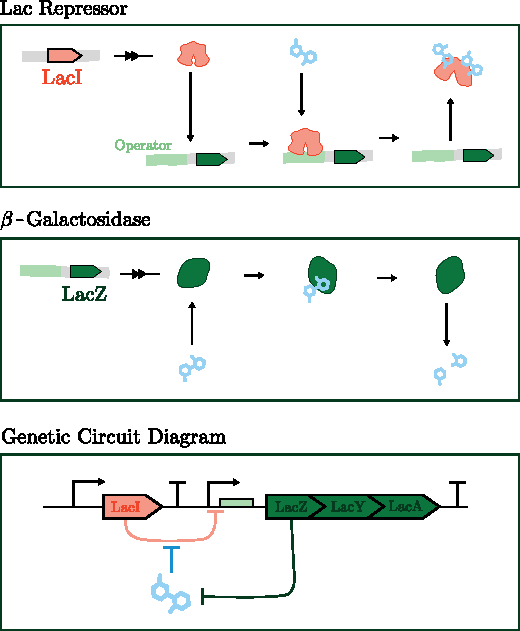
\includegraphics[scale=0.9]{lac-operon}
	\caption{Overview of the \emph{lac operon} }
	\label{fig:lac-operon}
\end{Figure}

Let us first consider what happens within a single cell of constant volume. We assume the rate $\alpha$ of transcription and translation of \emph{LacZ} into $\beta$-Gal is constant unless the operator region is blocked by \emph{LacR}. The repressor is inactivated by the binding of two (allo)lactose molecules $\ce{C12H22O11}$.

\begin{align*}
	\ce{
	\bond{~}Operator\bond{~}LacZ\bond{~} &->[$\alpha$]
	\bond{~}Operator\bond{~}LacZ\bond{~} + $\beta$-Gal \\
	C12H22O11 &->[$\beta$-Gal][+H2O] C6H12O6 + C6H12O6 \\
	\bond{~}Operator\bond{~}LacZ\bond{~} + LacR &<=>[k] \bond{~}Operator^\prime\bond{~}LacZ\bond{~} \\
	LacR + 2C12H22O11 &<=>[k^\prime] LacR^\prime}
\end{align*}
Proteins degrade over some finite half-life $\mu$ we also have
\begin{align*}
	\ce{$\beta$-Gal ->[$\mu$] \emptyset}
\end{align*}

The equilibrium dissociation constants $k,k'$ define the binding affinity if \emph{LacR} to the operator and its effector respectively. Let rate $\beta$ be the rate of hydrolysis of lactose by $\beta$-Gal. These rates are determined by molecular details, some of which can be modulated with genetic engineering. Changing the promoter sequences, for example, can modulate the rate $\alpha$. Thus it makes sense to collect these rates into our model parameter $\theta=(\alpha,\beta,k,k')$. Let the concentration of the effector be the experimentally controlled condition $p=[\ce{C12H22O11}]$ and the remaining concentrations be collected in state vector $u=(\mathrm{LacZ},\mathrm{LacR},\mathrm{Gal})$.

From this set of reactions it is possible to write down a \emph{chemical master equation} \cite{Gillespie1992,Gillespie2007} whose \emph{mean field approximation} yields a set of ordinary differential equations of the form \eqref{eq:differential-equations} which are commonly referred to as \emph{reaction rate equations}. This procedure is equivalent to the mass-action assumption used in chemistry. We note that the two major assumptions here are: a thermodynamic limit where the number of molecules is sufficiently large such that correlations due to discreteness can be ignored and a sufficiently \emph{well mixed} cytoplasm so that we do not have to model space.

The \emph{reaction rate equations} for the Lac operon become
\begin{align}
\frac{d}{dt}\mathrm{LacR} =  \mathrm{LacR}^\prime-& \frac{p^2}{2} k^{\prime} \mathrm{LacR} +  \mathrm{LacZ}^\prime  - k \mathrm{LacR}\,\mathrm{LacZ} \label{eq:lacR}\\\nonumber
\frac{d}{dt}\mathrm{LacR}^\prime =  -  &\mathrm{LacR}^\prime + \frac{p^{2}}{2} k^{\prime} \mathrm{LacR} \\\nonumber\\
\frac{d}{dt}\mathrm{LacZ} = & \mathrm{LacZ}^\prime - k \mathrm{LacR}\,\mathrm{LacZ}
\label{eq:lacZ}\\\nonumber
\frac{d}{dt}\mathrm{LacZ}^\prime =  - & \mathrm{LacZ}^\prime + k \mathrm{LacR}\,\mathrm{LacZ} \\\nonumber\\
\frac{d}{dt} \mathrm{Gal}= &\alpha \mathrm{LacZ} - \mu\mathrm{Gal}\label{eq:Gal} \\\nonumber
\frac{dp}{dt} = 2 \mathrm{LacR}^\prime &-p^{2} k^{\prime} \mathrm{LacR} - \beta p\,\mathrm{Gal} 
\end{align}
We can see two mass conservations: the total concentration of the $\mathrm{LacZ}$ gene and total concentration of $\mathrm{LacR}$. We can write down the conservation laws normalised such that the total concentrations add up to one
\begin{align}
	\mathrm{LacR}+\mathrm{LacR}^\prime + \mathrm{LacZ}^\prime &=1
	\label{eq:mass-conservation}\\\nonumber
	\mathrm{LacZ}+\mathrm{LacZ}^\prime =1 &
\end{align}
Substituting conservation laws \eqref{eq:mass-conservation} into equations \eqref{eq:lacR} and \eqref{eq:lacZ} allows us to close them and solve for the fraction of unbound $\mathrm{LacZ}$ available for transcription
\begin{align}
	\mathrm{LacZ}(p) = \frac{1}{\frac{1}{2}+\sqrt{\frac{1}{4}+\frac{k}{1+\frac{1}{2}k^\prime p^2}}}
	\label{eq:lac-unbound}
\end{align}
This is a \emph{hill}-type term that yields a basal level of transcription $\mathrm{LacZ}(p=0)\sim k^{-\frac{1}{2}}$ saturates at $\mathrm{LacZ}(p\rightarrow\infty)=1$ with $k^\prime$ controlling the slope of the curve. We can now plot a vector field for equations \eqref{eq:Gal} (Figure \ref{fig:switch}) revealing the dynamics between (allo)lactose and $\beta$-Gal. We can see that for any initial concentration $p$ and basal concentration $\mathrm{Gal}^*$ the presence of $p$ stimulates more production of $\mathrm{Gal}$ which in turn decreases the concentration of $p\rightarrow 0$ at which point the basal expression $\mathrm{Gal}^*$ is reached again. This is the simplest example of \emph{gene regulation} in response to environmental conditions but there is nothing \emph{switch}-like about it. The \emph{lac operon} maintains a single point of homeostasis $(p^*,\mathrm{Gal}^*)$ defined by
\begin{align}
	\left.\frac{d}{dt}\mathrm{Gal}\right|_{p^*,\mathrm{Gal}^*} &= \alpha\mathrm{LacZ}(p^*) - \mu\mathrm{Gal}^* = 0
	\label{eq:gal-steady} \\
	\left.\frac{dp}{dt}\right|_{p^*,\mathrm{Gal}^*} &= -\beta p^*\mathrm{Gal}^* =0
	\label{eq:lactose-steady}
\end{align}

\begin{Figure}
	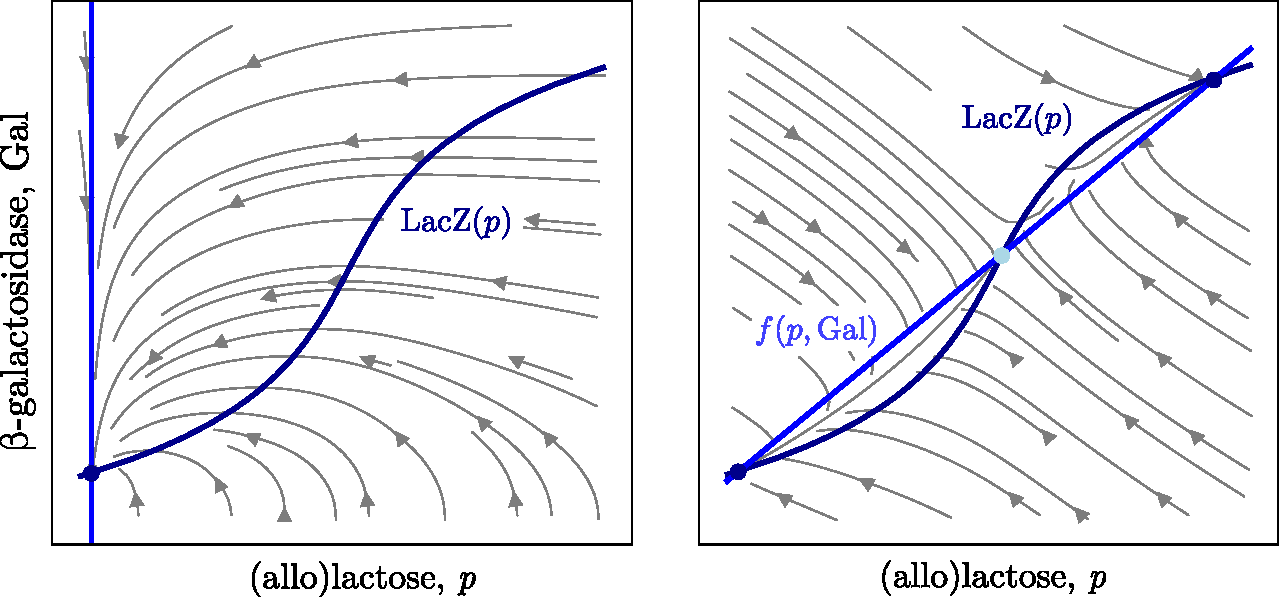
\includegraphics[scale=0.6]{switch}
	\caption{Monostable and bistable behaviour in the lac operon}
	\label{fig:switch}
\end{Figure}

In order to trigger the \emph{switch}-like behaviour we must engineer the dynamics defining the lactose \eqref{eq:lactose-steady} such that it defines a curve intersecting the \emph{hill}-type function three times (Figure \ref{fig:switch}). Mathematically we suppose there exists some $f(p,\mathrm{Gal})$ such that
\begin{align}
	\frac{dp}{dt} = -\beta p\mathrm{Gal} + f(p,\mathrm{Gal})
	\label{eq:lactose-control}
\end{align}
yields three intersections with equation \eqref{eq:gal-steady}. In practice $f$ can come from additional chemical reactions introduced by genetic engineering. We shall see how this was done with non-hydrolysable synthetic analogues of the \emph{lac operon} in Chapter \ref{chapter:double-exclusive}. The main take-away from this analysis is that whenever biochemical reactions yield \emph{hill}-type functions with inflection points, they tend to manifest on steady-state manifolds. This means that with  there is a good chance there exist chemical reactions that use it for its switching behaviour. In fact when the transglycosylation of lactose into \emph{allolactose} is taken into account, bistable behaviour is observed \cite{}.

Now that we've understood how genetic switches can manifest within a single cell, we can begin asking questions about populations of cells. We will do this again in the \emph{mean field approximation}, where a large population of cells can be described as a continuum of spatially extended concentrations $u(x,t)$. Some of molecules can be exchanges between cells, which gives rise to non-zero \emph{diffusion coefficients}, while others are confined within cells. As we shall see in Chapter \ref{chapter:double-exclusive}, a bistable region gives rise to sharp boundaries in gene expression. Such boundaries, their velocity and stability have been studied in the context of \emph{travelling wave solutions} of the \emph{Kolmogorov-Petrovsky-Piskunov equation} \cite{}.

\subsection{Self-organised Patterns \& Development}
During the development of any organism a hierarchy of self-organisation takes place that leads to the breaking of symmetry from a spherical cluster of undifferentiated cells to the formation of organ segments and limbs. This process is known as morphogenesis. Figure \ref{fig:morph}, taken from \cite{}, shows an example in which \textit{Hox} gene expression patterns in the body segments of Drosophila can drastically affect its development.

\begin{Figure}
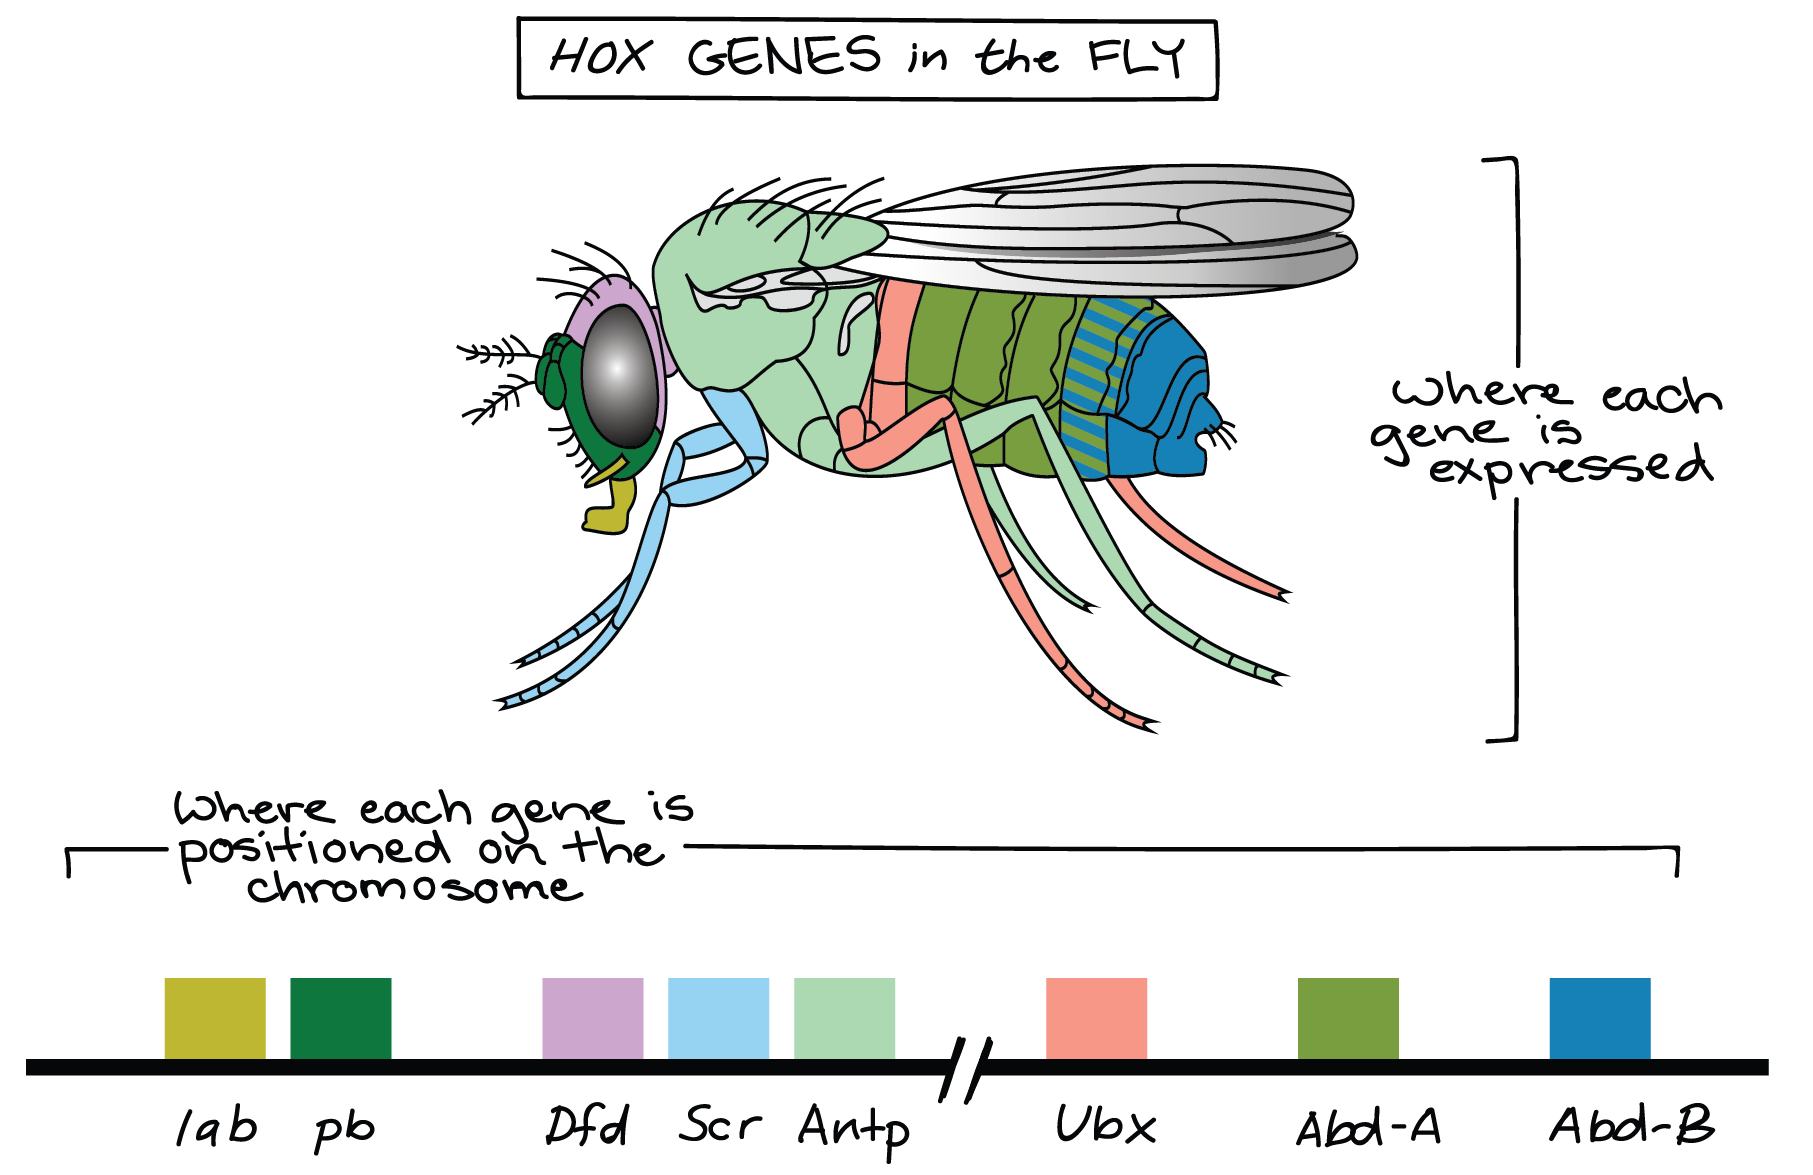
\includegraphics[width=90mm]{figures/morph1.png}\\
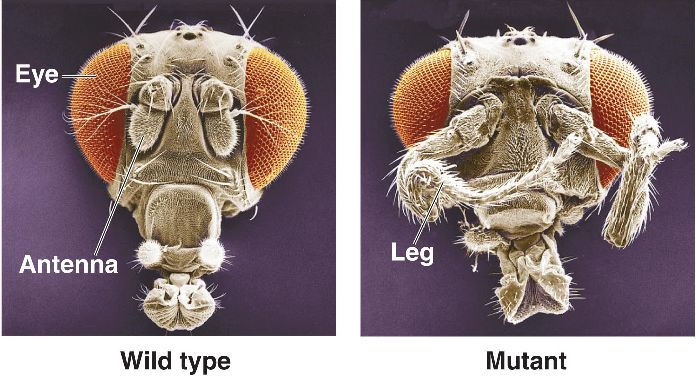
\includegraphics[width=90mm]{figures/morph2.png}
\caption{Top: \textit{Hox} gene expression patterns in body segments of drosophila Bottom: Mutation where legs grow in-place of antenna \cite{}}
\label{fig:morph}
\end{Figure}
\subsubsection{Morphogen-driven Patterns}
One of the central questions in developmental biology is how positional information is sensed by a population of cells and how sharp gene expression boundaries between populations are maintained for robust organ and body segment development. The French Flag model \cite{Wolpert1969PositionalDifferentiation.} proposes that cells have a threshold response to external signalling molecules -- henceforth referred to as morphogens -- which pre-pattern the organism from anterior to posterior and laterally. Some examples of morphogens include Wingless, Decapentaplegic and Sonic Hedgehog. Figure \ref{fig:gap} show the \textit{Gap} expression patterns that partition the Drosophila embryo into segments which are later differentiated by \textit{Hox} genes.

\begin{Figure}
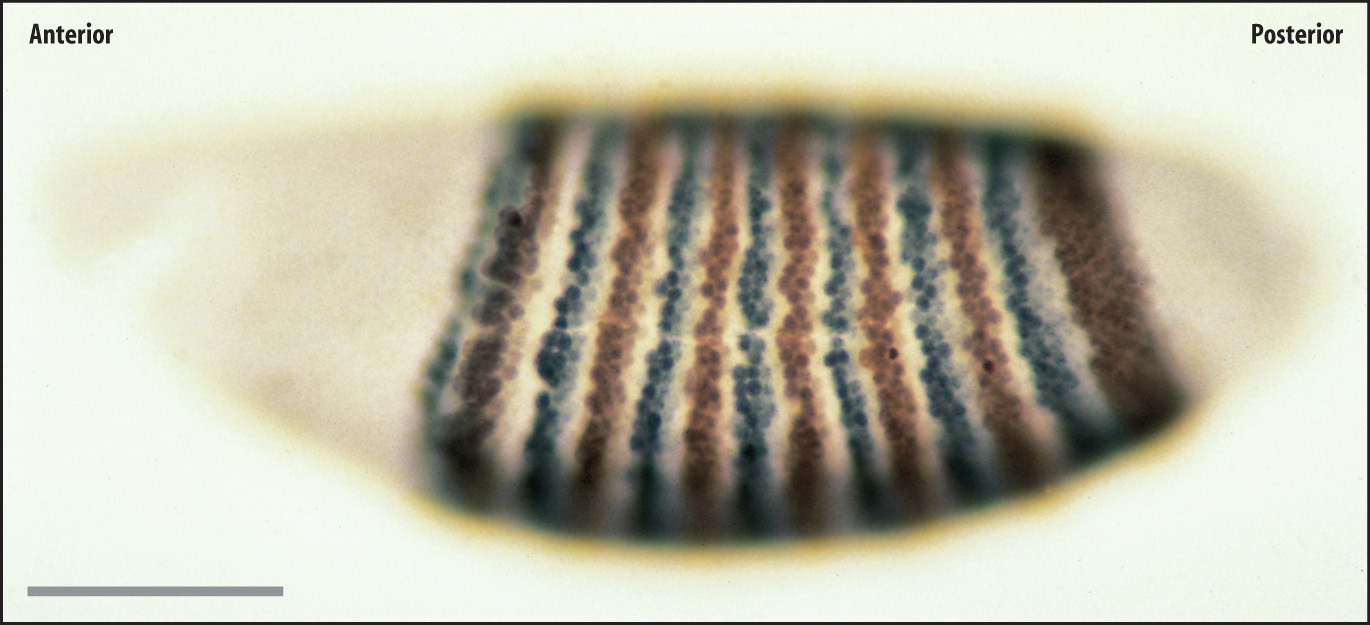
\includegraphics[width=90mm]{figures/gap.jpg}
\caption{Expression patterns of pair-rule \textit{Gap} genes in Drosophila embryo \cite{}}
\label{fig:gap}
\end{Figure}

\subsubsection{Self-organised Patterns}
How are morphogen gradients set up and maintained? How can they be robust against changes in size and geometry? A canonical example of self-organisation in bacteria is the quorum sensing system \cite{Miller2002QuorumBacteria}. Each cell secretes a signalling molecule resulting in the total concentration being proportional to the population density. This signal induces adaptive responses in metabolic and mobility in the whole colony. A long standing mathematical hypothesis that Turing patterns underlie self-organisation in cell populations. Recent literature suggests both morphogen-driven and Turing patterning mechanisms play a role in development \cite{Green2015PositionalCombine}

\begin{Figure}
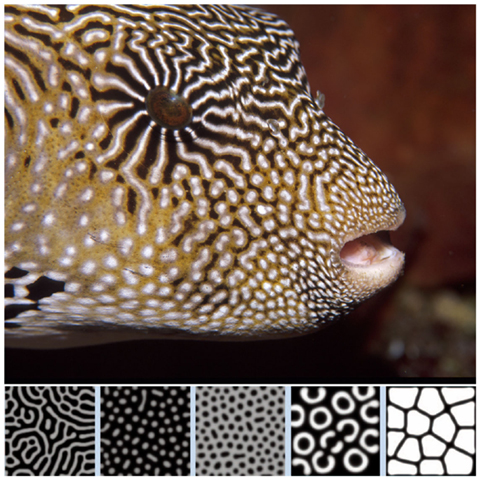
\includegraphics[width=70mm]{figures/turing.png}
\caption{Pigment patterns hypothesised to be generated by Turing mechanism}
\label{fig:turing}
\end{Figure}

\clearpage
\section{Phenotype Inference with Machine Learning}
\label{section:phenotype-inference}

Thus far we have outlined how applying bifurcation analysis to a model $\rates(u,p)$ relating the organism state $u$ to environmental conditions $p$ and genotype $\theta$ can be used to distinguish its phenotypes. What do we do in circumstances where the model is partially or completely unknown? In this case, rather than deriving the functional forms relating states $u$ from reasonable biochemical assumptions and mass-action laws, we rely on \emph{universal function approximators} \cite{}.
\begin{Figure}
    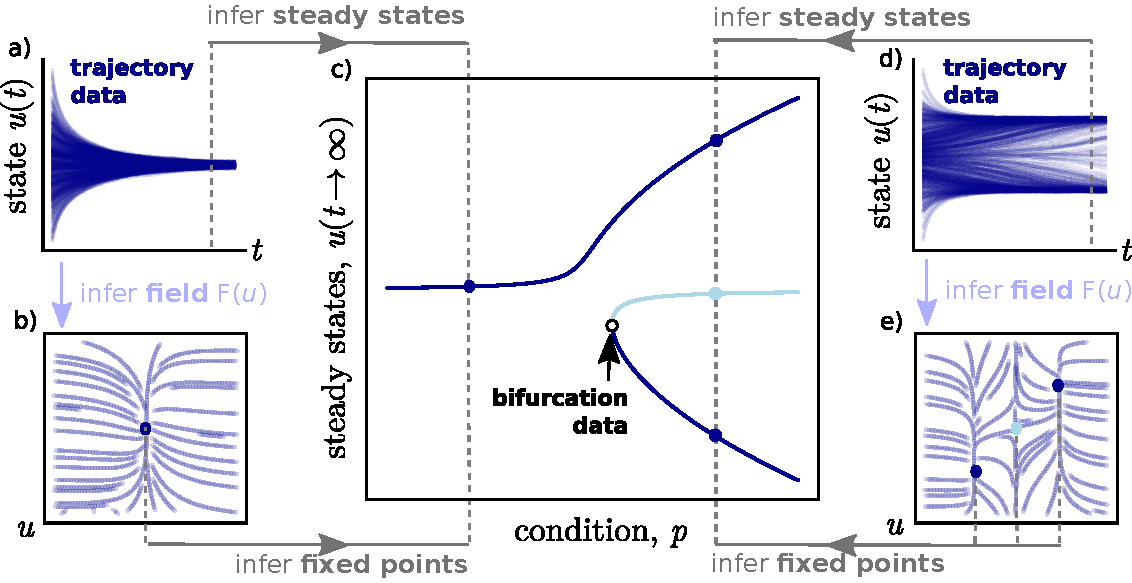
\includegraphics[width=14cm]{inferring-bifurcations}
    \caption{Bifurcation point extraction along the condition $p$ via two possible routes: steady state inference (a,d$\rightarrow$c) and fixed point inference (a,d$\rightarrow$b,e$\rightarrow$c). The fixed point inference route requires \emph{universal function approximator} $F(u)$ at different values of the condition $p$ and yields additional unstable fixed points.}
    \label{fig:inferring-bifurcations}
\end{Figure}
When a model $\rates(u,p)$ is absent it becomes difficult to know which observations to collect. In the era of high-throughput biology, the solution to this is to simply collect as many observations as possible and search the high-dimensional data for mechanisms that elucidate what the organism model could be. Such data may include flow cytometry, proteomics (MS/MS), transcriptomics (scRNA-seq) metabolomics (MS) and a wide variety of next-generation sequencing data \cite{}. Thus the problem of differentiating phenotypes becomes a matter of extracting bifurcations from high dimensional \emph{universal function approximators}.

Bifurcations along conditions $p$ can be extracted from data via two possible routes as depicted in Figure \ref{fig:inferring-bifurcations}: via a \emph{universal function approximator} $F(u)$ which enables the location of all fixed points, including unstable ones, or via direct inference from steady state data $u(t\rightarrow\infty)$. At best we could have state trajectory data $u(t)$ like single cell trajectories extracted via segmentation and tracking in fluorescence microscopy movies (for example the data acquired using the CellASIC ONIX Microfluidic Platform in Figure \ref{fig:double-exclusive:bistability}c). The majority of biomedical data is sparsely sampled with respect to time (for example the flow cytometry measurements in Figure \ref{fig:double-exclusive:flow-hysteresis} which were only collected at experiment end-points) and in such settings expecting to capture dynamical transients which would reveal the locations of unstable fixed points would be unreasonable. If we assume that the data was collected at a time where the organism is in homeostasis, then we can infer the steady states $u(t\rightarrow\infty)$ and any possible bifurcations directly from statistical measures of the data without needing a \emph{universal function approximator} $F(u)$. The emergent picture suggests a model of the state space $F(u)$ is desirable because it fully characterises the phenotype, but requires data or prior knowledge about dynamical transients of the organism. Fortunately, as we will see, statistics on the organism in homeostasis reveal stable steady states and static bifurcations.

\clearpage
\subsection{Phenotypes from Statistics in Homeostasis}
\label{section:steady-state-inference}
Suppose we collected a high dimensional single cell omics dataset $\dataset$ from an organism of genotype $\theta$ in various conditions $p$. We would like to know how many cell phenotypes there are in our dataset and how they may change in response to changes in environment $p$ or genetic manipulation $\theta$. Formally the data are a set of same size $|\dataset|$ as the number of cells, with an $N$-dimensional sample $U$ per cell. In practice there will be missing entries as not each cell will yield the same number or quality of observations. We assume that each sample is generated by a state distribution \eqref{eq:steady-state-distribution}. Not all cells share the same $\theta$ or even $p$ and this could give rise to an unknown number of clusters around a multitude of fixed points $\steady$ that could also depend on $\theta$ and $p$. We can write
\begin{equation}
	\dataset := \{ \,\, U \,\, | \,\,
	 \exists \theta,p :
	U \sim P_{\theta}(u,p) \}
\end{equation}
Since we can't possibly know the distribution $P_\theta$ because that would require knowing microscopic details and deriving a reasonable model $\rates$, we resort to dimensionality reduction in tandem with clustering methods to detect the phenotypes. To detect bifurcations look for regions of the data where the variance appears to diverge and we can use scaling laws from equation \eqref{eq:steady-state-distribution-near-fixed-point} to determine the type of bifurcation that is occurring and its corresponding degenerate direction.

\subsubsection{Impute, Reduce \& Cluster}
While the details of particular algorithms may vary, a popular pipeline for processing high dimensional biomedical data emerged: imputation of missing values followed by a combination of clustering and dimensionality reduction \cite{}. Imputation using \emph{nearest-neighbour methods} \cite{}, \emph{interpolation}  \cite{} or \emph{density sampling} \cite{} allow merging of datasets obtained from different experimental designs. Dimensionality reduction methods such as \emph{tSNE} \cite{} and \emph{UMAP} \cite{} are used to produce two dimensional overviews of datasets and are typically the first methods leveraged to get a feel for the global geometry of the high-dimensional point clouds. These methods also identify the highly variable feature combinations \cite{} as well noisy features that provide any information in distinguishing cell populations \cite{}. For a suitable choice of hyperparameters these maps reveal clusters and hence the number of distinct cell sub-populations. Clustering can then be used, either in the original high-dimensional space or the reduced space to segment the clouds \cite{}. Once the dataset is clustered, in principle we've identified the modes of the steady state distribution \eqref{eq:steady-state-distribution} and differential analysis \cite{} can be applied, together with domain knowledge, to distinguish whether any two clusters represent \emph{different phenotypes} or \emph{behavioural states} of the same phenotype.

\begin{Figure}
	{\phantomsubcaption\label{fig:impute}}
	{\phantomsubcaption\label{fig:reduce}}
	{\phantomsubcaption\label{fig:cluster}}
    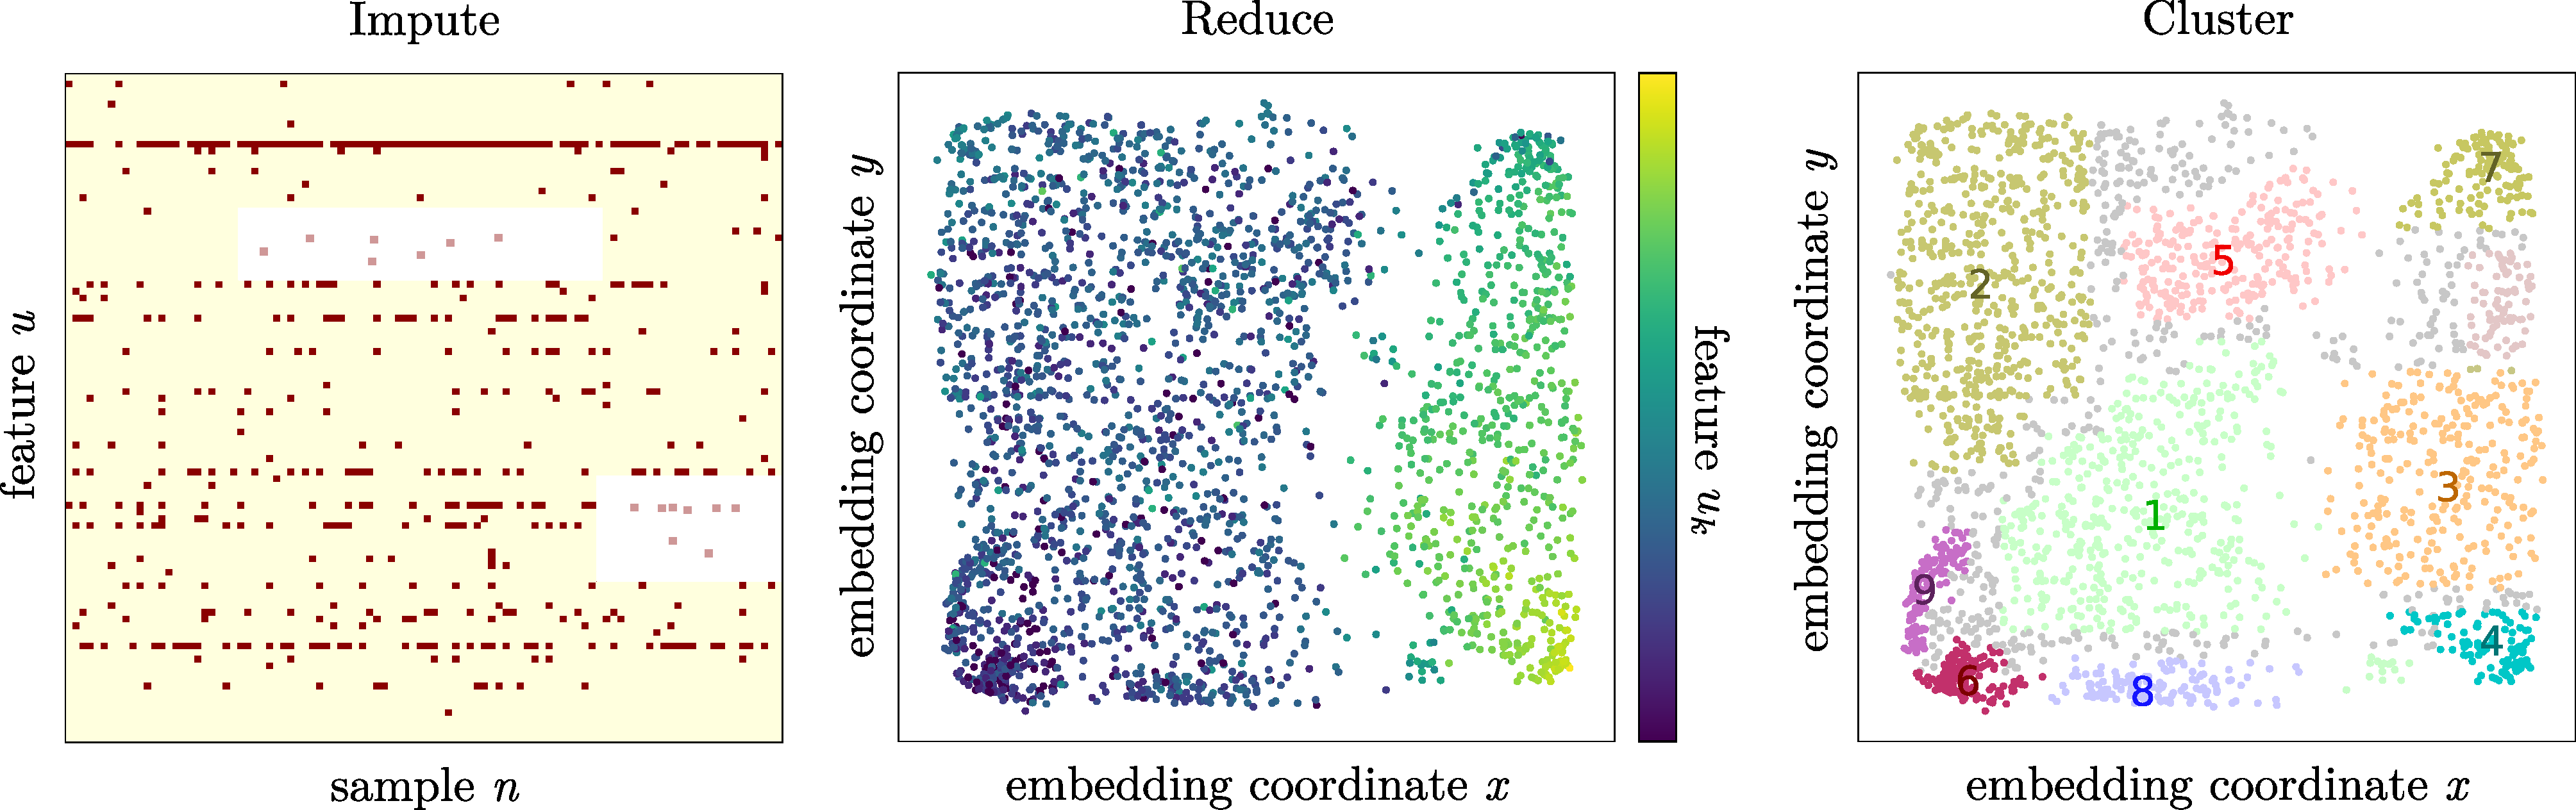
\includegraphics[width=14cm]{impute-reduce-cluster}
\begin{picture}(0,0)\put(-7,4.5){\subref{fig:impute}} \end{picture}
\begin{picture}(0,0)\put(-2.5,4.5){\subref{fig:reduce}} \end{picture}
\begin{picture}(0,0)\put(2.5,4.5){\subref{fig:cluster}} \end{picture}

    \caption{Overview of the impute, reduce \& cluster methods. \subref{fig:impute}. Heatmap of $N\times |\mathcal{U}|$ data matrix revealing regions of missing data that are imputed. \subref{fig:reduce}. Dimensionality reduction yielding an embedding which can be coloured by any feature $u_k$ to reveal differentials between regions. \subref{fig:cluster}. Clustering methods yield a segmentation of the dataset into populations that share features $u$}
    \label{fig:impute-reduce-cluster}
\end{Figure}

By looking at the variance within each cluster as we change $p$ we can also tell how close a population is to a bifurcation. This manifests as cluster splitting or merging with maximal variance at the splitting point. Unfortunately it would not be possible to distinguish whether a population is in a limit cycle or merely static, distributed across the states that make up the limit set. Therefore it is not possible to detect Hopf bifurcations from statistics in homeostasis.

Suppose we would like to detect saddle-node bifurcations within a bacterial cell population with respect to two experimental control conditions $p,p\prime\in\Reals$. We can set up a serial dilution along the columns for $p$ and along the rows for $p\prime$ in two 96-well plates. Cells allowed to grow in exponential phase in a finite concentration of either $p\ll p\prime$ or $p\gg p\prime$. Let us call this the \emph{priming} stage of the protocol as shown in Figure \ref{fig:cusp-sampling}a, resulting in two cell populations: $p$-primed cells and $p\prime$-primed cells. The priming concentrations must be chosen sufficiently high so that the resultant population states lie either side of a hypothesised cusp bifurcation. The two populations are transferred into separate 96-well plates containing the dilutions of $p,p'$; we call this the \emph{conditioning} stage in Figure \ref{fig:cusp-sampling}a.

\begin{Figure}
    \includegraphics[width=14cm]{hysteresis}
    \caption{Protocols (a) for extracting limit points with respect to conditions $p,p'$. Steady state distributions (b). Similarity measure (c)}
    \label{fig:cusp-sampling}
\end{Figure}

The cells are then transferred into a flow cytometer, gated for live singlets and processed with relevant compensation and auto-fluorescent normalisation, which would produce the population distributions $P(u)$ for the $p$-primed cells and $Q(u)$ for $p'$-primed cells in each well. By overlaying distributions $P(u),Q(u)$ for each well, a figure similar to Figure \ref{fig:cusp-sampling}b (or Figure \ref{fig:double-exclusive:flow-hysteresis}) can be produced. Finally, the limit points can be defined by a level set of distribution similarity measure $D(P||Q)$ in the $p,p\prime$-plane as shown in Figure \ref{fig:cusp-sampling}c. This similarity measure could be Kullback–Leibler divergence or something as simple as the distance between distribution medians. The level set must be some small positive amount $\epsilon$ above zero, picking out the onset of dissimilarity between steady state distributions $P(u)$ and $Q(u)$, and hence the onset hysteresis. We can define the limit points as
\begin{align}
    \targets = \{  (p,p\prime) : D(P||Q)=\epsilon, \epsilon>0 \} 
\end{align}

This approach may break down if multi-modal distributions exist in the data. This would be the case if something happened to prevent a sub-population of cells to switch from one state another other. Reasons for this could include too much cell burden or not enough time given for cells to reach a steady state. In this case, quantifying the efficiency of switching from either side of the cusp could be a quantity of interest.

This approach would not work for extracting dynamic bifurcations such as \emph{Hopf} since only steady state information is available. Furthermore, the accuracy of this method is subject to noise amplitude. This method works well for cases where changes in the number of stable steady states can be resolved in the measured steady state distributions.

\subsection{Phenotypes from Machine Learning Models}

Suppose we have the state as a function of time $u(t)$, sampled at sufficiently broad initial conditions $u(0)$. This would enable the estimation of field geometry $F(u)$ via \emph{universal function approximators} such as neural networks \cite{Chen2018NeuralEquations} and Gaussian processes \cite{Seeger2004GaussianLearning.}. We refer the reader to a modern review of the most successful machine learning approaches for designing \emph{universal function approximators} \cite{Bronstein2021GeometricGauges} where emphasis is made on understanding how group equivariant and group invariant transformations are stacked together. Note that we've dropped $\theta$ and $p$ from the \emph{universal function approximator}. We reserve $\theta$ to be a vector of biophysically meaningful parameters that make up an organism genotype. While \emph{universal function approximators} typically have a lot of parameters, they tend not to reveal the mechanism under study and hence cannot be used to deduce which genetic design interventions can be made.

In applications where the mechanism is partially known it is possible to combine the principled microscopic derivations of reaction rate model $\rates$ together with some \emph{universal function approximator} $F$. This is known as \emph{grey-box modelling} \cite{Meeds2019EfficientSystems}.

\subsubsection{Comparing Fields and Models}
% Non-parametric ___ using Gaussian Process regression
\label{section:field-inference}

In this early days of this thesis, we investigated whether it was possible to transform the time-domain data into state-space. This approach, and related works, are discussed in this section and can in principle be used with the microfluidic fluorescence microscopy data for parameter inference.

Consider we are given $K$ cell trajectories $\mathcal{D}_1$, $\mathcal{D}_2$ ... $\mathcal{D}_K$, each containing $N$ noisy observations of the state of the cell. Let the cell state be represented by state vector $u(t)\in\Reals^N$ which is hypothesized to obey a set of ordinary differential equations of the form \eqref{eq:differential-equations}. Instead of integrating the equations \eqref{eq:differential-equations} we would find an estimate for the derivative of the trajectories $\hat{f}$.

This is known as the \textit{smoothing} step \cite{Gugushvili2012Smoothing} should be done using unsupervised methods, for example with Gaussian Process Regressors \cite{Seeger2004GaussianLearning.} as shown in in Figure \ref{fig:inferred-cycles}. This requires the inversion of an $K'\times K'$ data matrix where $K':=\sum_k |\mathcal{D}_k|$ is the total number of trajectory data points. This has a computational complexity $K'^3$ which is only tractable with sparse datasets.

Let the region $\partial\mathcal{D}$ be a boundary defined by the Delaunay tessellation of the input data. Let us define the estimate $\hat f$ only within the region $\partial\mathcal{D}$ so that there are no extrapolation artefacts. For the Gaussian Process approach the estimate would be
\begin{equation}
    \hat{f}(u)\sim
        \mathcal{N}(\,\mu(u) ,\Matrix{\Sigma}(u)\,)
    \quad\mathrm{for}\quad u\in\partial\mathcal{D}
\end{equation}
\noindent where at any given state $u$ the field estimate $\hat{f}$ is generated by Gaussian distributions of mean vector $\mu$ and covariance matrix $\Matrix{\Sigma}$. Solving for these requires a choice of matrix-valued kernel function $\Matrix{K}(u,v)$ which encodes our knowledge about the local structure of the field. Sophisticated kernels for learning vector fields exist \cite{Fuselier2017ADecompositions} for decomposing fields in conservative and solenoidal components, which aid in localising fixed points and cycles.

The simplest choice of kernel assumes the components are independent and have a finite correlation length $\gamma$, such as Gaussian radial basis functions. Here $\Matrix{I}$ is the identity matrix and the hyperparameter $\gamma$ has to be optimised.
\begin{equation}
    \Matrix{K}(\Vector{u},\Vector{v}) = \Matrix{I}\,\mathbb{e}^{-\gamma|\Vector{u}-\Vector{v}|^2}
\end{equation}

The second step is called \textit{matching} where the estimated field $\hat{f}$ is used as an optimisation target against some parametrised function $\rates$ with unknown parameters $\theta$.

In our setting we would like to match the geometry of the field but not its magnitude; in this sense we are focusing on the qualitative aspects of the dynamics of a set of differential equations, rather than the quantitative dynamics or kinetics. This could be achieved with the following objective function
\begin{equation}
    \mathcal{L}(\theta|\mathcal{D}) := \e^{-\frac{\hat{f}\cdot\rates}
    {|\hat{f}||\rates|}}
	\label{eq:geometric-cost}
\end{equation}
\noindent where the cost is minimal when the data derivative $\hat{f}$ and the parametrised model $\rates$ point in the same direction and maximal when they point in opposing directions.

\begin{Figure}
    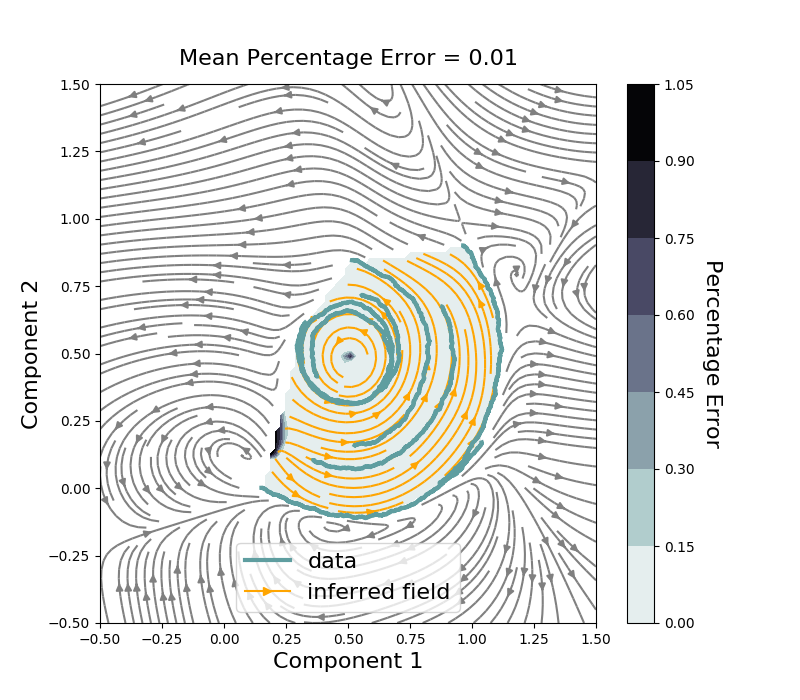
\includegraphics[width=125mm]{figures/cycle-2.png}
    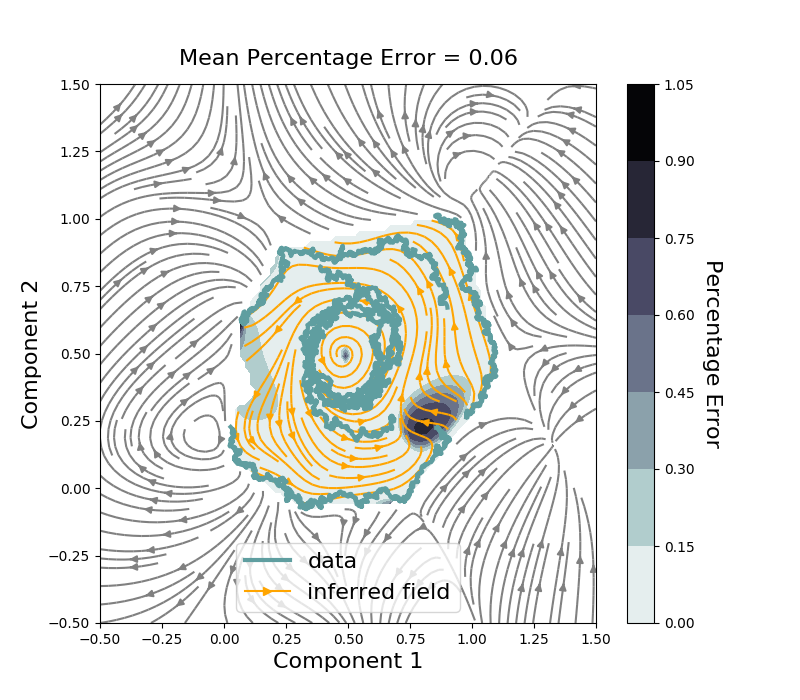
\includegraphics[width=125mm]{figures/cycle-1.png}
    \caption{Gaussian process regressors estimating derivative of the trajectories $\hat{f}$ from example trajectory datasets $\mathcal{D}_1$ ... $\mathcal{D}_K$ with varying signal to noise ratios. Interpolation error $E$ is shown as a heatmap; extrapolation fails}
    \label{fig:inferred-cycles}
\end{Figure}

Although we are getting close to focusing on qualitative features of a model, this objective function is still sensitive to the locations and shapes of fixed point and limit cycles. What if we cared about even higher-level features such as the number of fixed points? Or perhaps whether a system oscillates or not? This is where the language of bifurcation theory described in Chapter \ref{chapter:background} is optimally suited for this task, but fist we need to discuss how to set up experiments to detect bifurcations from flow cytometry data.

\begin{itemize}
    \item Vector field estimates too noisy to get bifurcation points?
    \item Divergence and the stability of fixed points
    \item curl and limit cycles. How does this relate to hopf example \ref{fig:inferred-cycles}
    \item Do we need a bistable example?
\end{itemize}

The accuracy of the cell trajectories is limited by cell segmentation and tracking algorithms. Initial investigations into this approach also suggested that trajectories need to be of sufficient temporal resolution and sampled from a wide variety of initial conditions. Such data is not widely available and ultimately we decided to focus on a method that could be used with a well-known workhorse in biomedical research: flow cytometry.




% We can then extract important state-space structures, such as stable and unstable fixed points, their eigenvalues $\lambda$, from the field geometry $F(u)$ at different values of the control condition $p$, and hence identify possible bifurcations.


% Data on steady states $u(t\rightarrow\infty)$ are more abundant and typically found in flow cytometry measurements. It is possible to infer the steady state manifold directly from such data (Figure \ref{fig:inferring-bifurcations} a,d$\rightarrow$c) but we would not be able to extract information on unstable fixed points or eigenvalues $\lambda$ of state-space structures. Since the criteria for bifurcations are not directly accessible, indirect measures (such as the population separation that can be seen in Figure \ref{fig:double-exclusive:flow-hysteresis}) must be used to extract bifurcations.


% \subsection{Classification and Regression}
% \begin{itemize}
%     \item Logistic regression
%     \item Nearest neighbour methods
%     \item Mixture Models
% \end{itemize}

% \subsection{Dimensionality Reduction Methods}
% \begin{itemize}
%     \item UMAP and Tsne
%     \item Sloppy parameters and identify-ability
% \end{itemize}

% \subsection{Clustering Methods}